%%____________________________________________________________________________||

%%____________________________________________________________________________||
\RCS$Revision: 339081 $
\RCS$HeadURL: svn+ssh://svn.cern.ch/reps/tdr2/notes/AN-XX-YYY/trunk/AN-XX-YYY.tex $
\RCS$Id: AN-XX-YYY.tex 339081 2016-04-18 15:39:58Z sakuma $

%%____________________________________________________________________________||
\newlength\cmsFigWidth
\ifthenelse{\boolean{cms@external}}{\setlength\cmsFigWidth{0.85\columnwidth}}{\setlength\cmsFigWidth{0.4\textwidth}}
\ifthenelse{\boolean{cms@external}}{\providecommand{\cmsLeft}{top\xspace}}{\providecommand{\cmsLeft}{left\xspace}}
\ifthenelse{\boolean{cms@external}}{\providecommand{\cmsRight}{bottom\xspace}}{\providecommand{\cmsRight}{right\xspace}}

%%____________________________________________________________________________||
\cmsNoteHeader{AN-XX-YYY}

%%____________________________________________________________________________||
\title{Simplified likelihood for public interpretation of results}

%%____________________________________________________________________________||
%\author[bristol]{R.~Aggleton}
% \author[imperial]{M.~Baber}
% \author[imperial]{R.~Bainbridge}
% \author[vub]{F.~Blekman}
% \author[imperial]{O.~Buchm\"uller}
% \author[bristol]{J.~Brooke}
% \author[imperial]{S.~Casasso}
\author[imperial]{M.~Citron}
\author[cern]{N.~Wardle}
% \author[imperial]{A.~Elwood}
% \author[bristol]{H.~Fl\"acher}
% \author[rochester]{A.~Garcia-Bellido}
% \author[imperial]{C.~Laner}
% \author[rochester]{K.H.~Lo}
% %\author[bristol]{C.~Lucas}
% \author[imperial]{S.A.~Malik}
% \author[imperial]{B.~Penning}
% \author[bristol]{T.~Sakuma}
% \author[vub]{D.~Smith^{1,}}
% \author[imperial]{A.~Tapper}

% \address[bristol]{University of Bristol, Bristol, UK}
\address[imperial]{Imperial College, London, UK}
\address[cern]{CERN, Geneva, CH}
% \address[vub]{Vrije Universiteit Brussel, Brussel, BE}
% \address[rochester]{University of Rochester, NY, US}

%%____________________________________________________________________________||
\date{\today}

%%____________________________________________________________________________||
\abstract{}

%%____________________________________________________________________________||
\hypersetup{ 
  pdfauthor={Matthew Citron.},
  pdftitle={Simplified likelihood for the re-interpretation of public CMS results.
  },
  pdfsubject={CMS,
  },
  pdfkeywords={CMS
  },
}

%%____________________________________________________________________________||
\maketitle

%%____________________________________________________________________________||
\tableofcontents

%%____________________________________________________________________________||
\newcommand{\kfactor}{\ensuremath{k\text{-factor}}\xspace}
\newcommand{\kfactors}{\ensuremath{k\text{-factors}}\xspace}
\newcommand{\njet}{\ensuremath{n_{\text{jet}}}\xspace}
\newcommand{\njetlow}{\ensuremath{2 \leq \njet \leq 3}\xspace}
\newcommand{\njethigh}{\ensuremath{\njet \geq 4}\xspace}
\newcommand{\nb}{\ensuremath{n_{\text{b}}}\xspace}
\newcommand{\alphat}{\ensuremath{\alpha_{\text{T}}}\xspace}
\newcommand{\alphatcut}{\ensuremath{\alpha_{\text{T}}^{\text{cut}}}\xspace}
\newcommand{\htalphat}{\texttt{HT\_AlphaT}\xspace}
\newcommand{\htcat}{\ensuremath{\HT^{\text{cat}}}\xspace}
\newcommand{\photon}{\texttt{Photon}\xspace}
\newcommand{\muht}{\texttt{Mu\_HT}\xspace}
\newcommand{\httrigger}{\texttt{HT}\xspace}
\newcommand{\mt}{\ensuremath{M_{\textrm T}}\xspace}
\newcommand{\gj}{\ensuremath{\gamma} + jets\xspace}
\newcommand{\mj}{\ensuremath{\mu} + jets\xspace}
\newcommand{\mmj}{\ensuremath{\mu\mu} + jets\xspace}
\newcommand{\lj}{\ensuremath{\ell} + jets\xspace}
\newcommand{\llj}{\ensuremath{\ell\ell} + jets\xspace}
\newcommand{\ej}{\ensuremath{e} + jets\xspace}
\newcommand{\eej}{\ensuremath{ee} + jets\xspace}
\newcommand{\npre}{\ensuremath{N_{\textrm{pred}}}\xspace}
\newcommand{\nobs}{\ensuremath{N_{\textrm{obs}}}\xspace}
\newcommand{\njets}{\ensuremath{N_{\textrm{jet}}}\xspace}
\newcommand{\sq}{\ensuremath{\tilde{\rm q}}\xspace}
\newcommand{\st}{\ensuremath{\tilde{\rm t}}\xspace}
\newcommand{\gl}{\ensuremath{\tilde{\rm g}}\xspace}
\newcommand{\dht}{\ensuremath{\Delta\scalht}\xspace}
\newcommand{\dEt}{\ensuremath{\Delta\Et}\xspace}
\newcommand{\ewk}{\ensuremath{\mathrm{EWK}}\xspace}
\newcommand{\qcd}{\ensuremath{\mathrm{QCD}}\xspace}
\newcommand{\fZinv}[1]{\ensuremath{f_{\rm Zinv}^{#1}}\xspace}
\newcommand{\zInv}[1]{\ensuremath{Z_{\rm inv}^{#1}}\xspace}
\newcommand{\meanHt}[1]{\ensuremath{\langle \HT \rangle^{#1}}\xspace}
\newcommand{\lk}[2]{\ensuremath{L^{\rm #1}_{\rm #2}}\xspace}
\newcommand{\sep}{\ensuremath{68^{\mathrm{th}}}\xspace}
\newcommand{\partonht}{\ensuremath{\scalht^{\rm parton}}\xspace}
\newcommand{\meff}{\ensuremath{M_{\rm eff}}\xspace}
\newcommand{\mhttt}{\ensuremath{\hslash_{\rm T}^{TT}}\xspace}
\newcommand{\ifb}{\ensuremath{\text{fb}^{-1}}\xspace}
\newcommand{\ipb}{\ensuremath{\text{pb}^{-1}}\xspace}
\newcommand{\DMtt}{DM\ensuremath{+t\bar{t}}\xspace}
\newcommand{\DMj}{DM\ensuremath{+\rm{jet}}\xspace}
\newcommand{\DMbb}{DM\ensuremath{+b\bar{b}}\xspace}
\newcommand{\mchi}{\ensuremath{m_{\chi}}\xspace}
\newcommand{\mphi}{\ensuremath{M_{\Phi}}\xspace}
\newcommand{\pchi}{\ensuremath{\chi}\xspace}
\newcommand{\pphi}{\ensuremath{\Phi}\xspace}
\newcommand{\gsm}{\ensuremath{g_{\textrm{SM}}}\xspace}
\newcommand{\gdm}{\ensuremath{g_{\textrm{DM}}}\xspace}

\newcommand\rs{\raisebox{1.0ex}[-1.0ex]}
\newcommand{\ra}{\ensuremath{\rightarrow}}
\newcommand{\znunu}{\ensuremath{{\text Z} \ra \nu\bar{\nu}}\xspace}
\newcommand{\zll}{\ensuremath{{\text Z} \ra \ell\ell}\xspace}
\newcommand{\zmumu}{\ensuremath{{\text Z} \ra \mu\mu}\xspace}
\newcommand{\zee}{\ensuremath{{\text Z} \ra ee}\xspace}
\newcommand{\wmunu}{\ensuremath{{\text W} \ra \mu\nu}}
\newcommand{\wtaunu}{\ensuremath{{\text W} \ra \tau\nu}}
\newcommand{\dphi}{\ensuremath{\Delta \phi}}
\newcommand{\dphijj}{\ensuremath{\Delta \phi_{ j1,j2}}}
\newcommand{\Pt}{\ensuremath{{p_{\text T}}}\xspace}
\newcommand{\pts}{\ensuremath{p_{\text T}{\text s}}\xspace}
\newcommand{\Et}{\ensuremath{{E_{\text T}}}\xspace}
\newcommand{\ptjf}{\ensuremath{p_{\rm T}^{ {\rm j}_1} }}
\newcommand{\ptjs}{\ensuremath{p_{\rm T}^{ {\rm j}_2} }}
\newcommand{\ptjt}{\ensuremath{p_{\rm T}^{ {\rm j}_3} }}
\newcommand{\etajf}{\ensuremath{\eta^{ {\rm j}_1} }}
\newcommand{\etajs}{\ensuremath{\eta^{ {\rm j}_2} }}
\newcommand{\etajt}{\ensuremath{\eta^{ {\rm j}_3} }}
\newcommand{\ttj}{\ensuremath{\rm{t}\bar{\rm{t}} + jets}\xspace}
\newcommand{\wj}{\ensuremath{\rm W + \textrm{jets}}\xspace}
\newcommand{\wej}{\ensuremath{{\rm W}(\rightarrow{\rm e}\nu) + \textrm{jets}}\xspace}
\newcommand{\wmj}{\ensuremath{{\rm W}(\rightarrow\mu\nu) + \textrm{jets}}\xspace}
\newcommand{\zj}{\ensuremath{{\rm Z} + \textrm{jets}}\xspace}
\newcommand{\zmmj}{\ensuremath{{\rm Z}(\rightarrow\mu\mu) + \textrm{jets}}\xspace}
\newcommand{\zeej}{\ensuremath{{\rm Z}(\rightarrow{\rm ee}) + \textrm{jets}}\xspace}

\newcommand{\al}{\ensuremath{\alpha}}
\newcommand{\alt}{\ensuremath{\alpha_{\text{T}}}\xspace}
\newcommand{\etaabs}{\ensuremath{|\eta|}}
%\newcommand{\gev}{\ensuremath{\mathrm{\,Ge\kern -0.1em V}}}
\newcommand{\pb}{\ensuremath{pb^{-1}}}
\newcommand{\mjj}{\ensuremath{M_{\text{inv}}^{j1,j2}}}
%\newcommand{\ttbar}{\ensuremath{t\bar{t}}}
\newcommand{\chiznew}{\ensuremath{\chi^{0}}\xspace}
\newcommand{\chipnew}{\ensuremath{\chi^{+}}\xspace}
%\newcommand{\chipm}{\ensuremath{\chi^{\pm}}\xspace}
\newcommand{\sQuanew}{\ensuremath{\tilde{\rm q}}\xspace}
\newcommand{\sGlunew}{\ensuremath{\tilde{\rm g}}\xspace}
\newcommand{\ttNew}{\ensuremath{\rm{t}\bar{\rm{t}}}\xspace}
\newcommand{\tev}{\TeV}
%<TW date="30/10/2010">
%\newcommand{\Et}{E_{T}}
\newcommand{\combIso}{Iso_{\textrm{comb.}}}
\renewcommand{\arraystretch}{1.2}
\newcommand{\bigNum}[2]{#1 \, \times \, 10 \, ^{#2}}
%</TW>

\newcommand{\raT}{\ensuremath{R_{\alt}}}
\newcommand{\RaT}{\ensuremath{R_{\alt}}\xspace}

\newcommand{\Ttwocc}{\ensuremath{\text{pp}\,\ra\,\sTop\sTop^{*}\,\ra\,\text{c}\chiz\,\bar{\text{c}}\chiz}}
\newcommand{\Ttwotc}{\ensuremath{\text{pp}\,\ra\,\sTop\sTop^{*}\,\ra\,\text{t}\chiz\,\bar{\text{c}}\chiz}}
\newcommand{\Ttwodegen}{\ensuremath{\text{pp}\,\ra\,\sTop\sTop^{*}\,\ra\,\text{b}ff'\chiz \,\text{b}ff'\chiz}}
\newcommand{\Ttwobw}{\ensuremath{\text{pp}\,\ra\,\sTop\sTop^{*}\,\ra\,\text{b}W\chiz \,\bar{\text{b}}W\chiz}}
\newcommand{\Ttwott}{\ensuremath{\text{pp}\,\ra\,\sTop\sTop^{*}\,\ra\,\text{t}\chiz\,\bar{\text{t}}\chiz}}
\newcommand{\Ttwobb}{\ensuremath{\text{pp}\,\ra\,\sBot\sBot^{*}\,\ra\,\text{b}\chiz\,\bar{\text{b}}\chiz}}
\newcommand{\Ttwoqq}{\ensuremath{\text{pp}\,\ra\,\sQua\sQua^{*}\,\ra\,\text{q}\chiz\,\bar{\text{q}}\chiz}}
\newcommand{\Tonebbbb}{\ensuremath{\text{pp}\,\ra\,\sGlunew\sGlunew^{*}\,\ra\,\bar{\text{b}}\text{b}\chiz\,\bar{\text{b}}\text{b}\chiz}}
\newcommand{\Toneqqqq}{\ensuremath{\text{pp}\,\ra\,\sGlunew\sGlunew^{*}\,\ra\,\bar{\text{q}}\text{q}\chiz\,\bar{\text{q}}\text{q}\chiz}}
\newcommand{\Tonetttt}{\ensuremath{\text{pp}\,\ra\,\sGlunew\sGlunew^{*}\,\ra\,\bar{\text{t}}\text{t}\chiz\,\bar{\text{t}}\text{t}\chiz}}
\newcommand{\Tonettbb}{\ensuremath{\text{pp}\,\ra\,\sGlunew\sGlunew^{*}\,\ra\,\bar{\text{t}}\text{t}\chiz\,\bar{\text{b}}\text{b}\chiz}}

\newcommand{\ppToGluGlu}{\ensuremath{\text{pp}\,\ra\,\sGlunew\sGlunew^{*}}}
\newcommand{\chipmToWNo}{\ensuremath{\chipm \,\ra\,W^{\pm}\chiz}}
\newcommand{\gluToBBNo}{\ensuremath{\sGlunew\,\ra\,\bar{\text{b}}\text{b}\chiz}}
\newcommand{\gluToTTNo}{\ensuremath{\sGlunew\,\ra\,\bar{\text{t}}\text{t}\chiz}}
\newcommand{\gluToQQNo}{\ensuremath{\sGlunew\,\ra\,\bar{\text{q}}\text{q}\chiz}}
\newcommand{\gluToTBAll}{\ensuremath{\sGlunew\,\ra\,\text{t}\text{b}\chipm(W^{\pm}\chiz)/\bar{\text{t}}\text{t}\chiz/\bar{\text{b}}\text{b}\chiz}}
\newcommand{\gluToTBWNo}{\ensuremath{\sGlunew\,\ra\,\text{t}\text{b}\chipm, \chipmToWNo}}
\newcommand{\gluToTStop}{\ensuremath{\sGlunew\,\ra\,\text{t}\sTop}}
\newcommand{\ppToStopStop}{\ensuremath{\text{pp}\,\ra\,\sTop\sTop^{*}}}
\newcommand{\stopToTNo}{\ensuremath{\sTop\,\ra\,\text{t}\chiz}}
\newcommand{\stopToCNo}{\ensuremath{\sTop\,\ra\,\text{c}\chiz}}
\newcommand{\stopToBWNo}{\ensuremath{\sTop\,\ra\,\text{b}\chipm,\chipmToWNo}}
\newcommand{\stopToBFFNo}{\ensuremath{\sTop\,\ra\,\text{b}ff'\chiz}}
\newcommand{\stopToMixed}{\ensuremath{\sTop\,\ra\,\text{c}\chiz/\text{b}ff'\chiz}}
\newcommand{\stopToTB}{\ensuremath{\sTop\,\ra\,\text{t}\chiz/\text{b}\chipm,\chipmToWNo}}
\newcommand{\stopToBW}{\ensuremath{\sTop\,\ra\,\text{b}\chipm,\chipmToWNo}}
\newcommand{\ppToSbotSbot}{\ensuremath{\text{pp}\,\ra\,\sBot\sBot^{*}}}
\newcommand{\sbottomToB}{\ensuremath{\sBot\,\ra\,\text{b}\chiz}}
\newcommand{\ppToSquaSqua}{\ensuremath{\text{pp}\,\ra\,\sQua\sQua^{*}}}
\newcommand{\squarkToQ}{\ensuremath{\sQua\,\ra\,\text{q}\chiz}}

\newcommand\T{\rule{0pt}{2.6ex}}
\newcommand\B{\rule[-1.2ex]{0pt}{0pt}}

\def\eslash{{\hbox{$E$\kern-0.6em\lower-.05ex\hbox{/}\kern0.10em}}}
\def\vecmet{\mbox{$\vec{\eslash}_T$}} %missing ET vector
\def\vecet{\mbox{$\vec{E}_\text{T}$}} % ET vector
\def\MET{\mbox{$\eslash_\text{T}$}\xspace}
%\def\met{\mbox{$\eslash_\text{T}$}\xspace}
\def\met{\mbox{$E_\text{T}^{\rm miss}$}\xspace}
\def\pfmet{\mbox{$\eslash_\text{T}^{\rm PF}$}\xspace}
\def\mex{\mbox{$\eslash_\text{x}$}} %missing Ex
\def\mey{\mbox{$\eslash_\text{y}$}} %missing Ey
\def\mepar{\mbox{$\eslash_\parallel$}}
\def\meperp{\mbox{$\eslash_\perp$}}
\def\Zmm{Z \rightarrow \mu\mu}
\def\metvec{\mbox{$\vec{\met}$}\xspace}
\def\metvecrec{\mbox{$\vec{\met}^{\rm rec}$}\xspace}
\def\metvecgen{\mbox{$\vec{\met}^{\rm gen}$}\xspace}
\def\metgen{\mbox{$\met^{\rm gen}$}\xspace}
\def\metparl{\mbox{$\mepar^{\rm rec}$}\xspace}
\def\metperp{\mbox{$\meperp^{\rm rec}$}\xspace}
\def\deltamet{\mbox{$\Delta\met$}\xspace}
\def\pthat{\mbox{$\hat{p}_T$}\xspace}
\def\hslash{{\hbox{$H$\kern-0.8em\lower-.05ex\hbox{/}\kern0.10em}}}
\def\MHT{\mbox{$\hslash_\text{T}$}\xspace}
%\def\mht{\mbox{$\hslash_\text{T}$}\xspace}
\def\mht{\mbox{$H_{\rm T}^{\rm miss}$}\xspace}
\def\mhtvec{\mbox{$\vec{H}_{\rm T}^{\rm miss}$}\xspace}
%\def\mhtmet{\mbox{$\hslash_\text{T} / \eslash_\text{T}$}\xspace}
\def\mhtmet{\mbox{$\mht / \met$}\xspace}
\def\mhtmetmiss{\mbox{$\H_\text{T}^{\rm miss} / \E_\text{T}^{\rm miss}$}\xspace}
%\def\rmhtmet{\mbox{$R_{\hslash_\text{T} / \eslash_\text{T}}$}\xspace}
\def\rmhtmet{\mbox{$R_{\mht / \met}$}\xspace}
\def\sumet{\mbox{$\sum \rm{E}_\text{T}$}\xspace}
\def\scalht{\mbox{$H_\text{T}$}\xspace}
\def\etmiss{\mbox{$\eslash_\text{T}$}\xspace}
\def\htmiss{\mbox{$\hslash_\text{T}$}\xspace}
\def\mtt{\mbox{$\rm{M}_\text{T2}$}\xspace}
\def\rmec{\mbox{$R_{\mht/\met}$}\xspace}
\def\bdphi{\mbox{$\Delta\phi^{*}_{\rm min}$}\xspace}
\def\dphimhtj{\mbox{$\Delta\phi(j_{1234}, \mht)_{\rm min}$}\xspace}
\def\dphimhtjall{\mbox{$\Delta\phi(j_{all}, \mht)_{\rm min}$}\xspace}
\def\bigeslash{{\hbox{$E$\kern-0.38em\lower-.05ex\hbox{/}\kern0.10em}}}
\def\bigmet{\mbox{$\bigeslash_T$}}
\def\bighslash{{\hbox{$H$\kern-0.6em\lower-.05ex\hbox{/}\kern0.10em}}}
\def\bigmht{\mbox{$\bighslash_T$}}
\def\incl{\includegraphics[width=0.49\linewidth]}
\def\inclrot{\includegraphics[angle=90,width=0.47\linewidth]}
\def\INCL{\includegraphics[angle=90,width=0.45\linewidth]}
\def\Incl{\includegraphics[angle=90,width=0.60\linewidth]}
\def\cls{\mbox{CL$_s$}\xspace}
\def\nj{\ensuremath{n_{\mathrm{jet}}}}
\def\nb{\ensuremath{n_{\mathrm{b}}}}

\newcommand{\zero}{\ensuremath{\phantom{0}}}


%%____________________________________________________________________________||
%%____________________________________________________________________________||
\section{Introduction}
\label{sec:intro}

Searches for new physics beyond the standard model (BSM) by the CMS collaboration are performed using a wide variety of 
strategies and using events with different final states and kinematic properties.  Often, 
the results of these searches are presented in terms of ``model-independent'' limits on the production 
cross-section for some new BSM particle. Common examples are searches for resonances whose decay products 
can be experimentally reconstructed with a high resolution resulting in narrow invariant mass peaks which can be readily distinguished from 
a smoothly varying background~\cite{Khachatryan:2016yec}. Several searches, however, involve the use of final states with low mass resolution or involving 
quantities such as the missing transverse momentum (as in~\cite{Khachatryan:2011tk,Khachatryan:2016mdm}) or the angles between objects in the final state (as in~\cite{Khachatryan:2015pua}). 
These searches are typically performed using the 
distributions of these quantities for which the separation between standard model (SM) processes and BSM signals is limited. Furthermore, 
sensitivity to a wide range of BSM physics can often be improved using a categorisation of events based on the number of a particular 
object in the event, such as charged leptons or jets, or based on a multivariate analysis (MVA) of the kinematics and/or reconstruction and 
identification quality of the final state particles in the event. For such searches, limits can only be expressed in terms of the 
parameter space of some specific complete or simplified BSM model.

Searches for BSM physics are often interpreted using a small subset of new physics 
models serving as benchmarks for the sensitivity of the search. Often, the searches are re-interpreted 
to provide constraints on other models of new physics, not included in the publication.
Re-interpretations can also be provided using complete models of new physics and the constraints from 
these searches are combined with measurements and searches from other experiments~\cite{mastercode}. 
For these reinterpretations, the signal contribution is typically determined using an event generator 
such as {\sc Pythia}~\cite{pythia} followed by a simulation of the detector 
response and resolution using tools such as {\sc Delphes}~\cite{delphes} or by matching generated particles to
the reconstructed objects according to published information regarding the performance of the CMS detector. 
The background contributions to search regions and the associated systematic uncertainties, however, often rely
on simplifying assumptions, in particular where the search is performed using multiple event categories or 
the distributions of one or more discriminating variables, which can lead to inaccuracies in the re-interpretation. 

In previous publications, the total background predictions  
and systematic uncertainty has been provided by searches in each region for which the contribution 
from potential BSM signals are expected to be significant. 
Typically these searches also define 'super' regions which cover larger regions of the relevant discriminating variables 
than those used in the analysis. This allows re-interpretation of the results by selecting the most sensitive 
super region for a given BSM interpretation. This procedure avoids the need to provide correlations between the 
distributions of the discriminating variables. While the procedure is robust, the loss of information included in the regions 
neglected for each BSM scenario can can result in a significant loss of sensitivity. 

In this note, an alternative procedure for re-interpreting BSM physics searches by approximating
the full background model and systematic uncertainties is presented. The procedure uses a reduced 
set of information to describe the background model 
and the correlations between different regions used in the searches, minimising the loss of sensitivity.
The following key points will be discussed in this note;

\begin{itemize}

\item Many BSM CMS searches are sensitive to BSM models not discussed in
the corresponding CMS publications.

\item Often these searches are based on the distribution of one or more 
discriminating variables and commonly performed using event counts 
in many disjoint search regions.  Although the event counts, background
expectations, and background uncertainties are provided for each search region,
reinterpretation of the results in different contexts is not possible
without knowledge of the full background model.

\item A key ingredient for reinterpretations is the ability to predict
the number of events expected in each search region for a given BSM model.
Details of this procedure are not in the scope of this document.

\item To facilitate reinterpretation CMS can make available an
approximate covariance matrix for the background in the 
various search regions, or a reduced set thereof.

\item This covariance matrix can then be used to build a simplified
likelihood for any signal model, as described in Section 2.1.

\item Based on this likelihood, one can extract approximate limits
on BSM models not considered in the original CMS publication under 
a number of different statistical treatments, the choice of which 
is left to the user.

\item Alternatively, for simplicity, the user may decide to define
their own single search region tailored to the BSM model of interest.  
Provided this single search is defined as the union of a number of analysis
search regions, the covariance matrix can be used to extract the total uncertainty
on the background expectation in the single search region.

\item It should be emphasized that reinterpretations using the simplified procedures 
outlined in this note can only approximate the result of a full CMS
analysis, due the imperfections in estimating the BSM
acceptance from simplified detector models and the underlying assumptions of the 
procedure itself.

\end{itemize} 


%%____________________________________________________________________________||

%%____________________________________________________________________________||
\section{Simplified likelihood}
\label{sec:simplified-likelihood}

While several methods for extracting 
limits are used, the most common approach follows the frequentist paradigm using the procedure 
described in Refs.~\cite{} and ~\cite{}. 
The observed data are interpreted using a likelihood defined as,

\begin{equation}
 \mathcal{L}(\mu, \boldsymbol{\theta}) = 
 \mathcal{P}(\mathrm{data}|\mu\cdot s(\boldsymbol{\theta}) + b(\boldsymbol{\theta})) \cdot p(\tilde{\boldsymbol{\theta}}|\boldsymbol{\theta})
\label{eq:generic-likelihood}
\end{equation}

where $\mathcal{P}(\mathrm{data}|\mu\cdot s(\boldsymbol{\theta}) + b(\boldsymbol{\theta}))$ is a product of the proability 
over all events or bins in one or more discriminating variables or event categories to observe the data. The parameters 
$\boldsymbol{\theta}=\left(\theta_{1},\theta_{2}...\right)$ are nuisance parameters, which are used to model the variation of the 
signal $s(\boldsymbol{\theta})$ and background $b(\boldsymbol{\theta})$ models due to systematic uncertainties. Often, these nuisance 
parameters are constrained by external measurements, $\tilde{\boldsymbol{\theta}}$, which are encoded in the 
probability density function $p(\tilde{\boldsymbol{\theta}}|\boldsymbol{\theta})$. 
The parameter $\mu$, typically referred to as a signal strenth, is a common scale factor for the expected signal contribution. 
A particular BSM model predicting $s(\boldsymbol{\theta})$ is said to be excluded at some confidence level 
when every value of $\mu\ge1$ is excluded at at least that confidence level.

In order to acheive a good senstivity to a wide range of BSM models, searches are often performed 
by categorising events with different final states or according to some discriminating variable. 
The precise modelling of the backgrounds can therefore be rather complicated, involving many 
nuisance parameters. For this reason, the full likelihood is therefore often 
too detailed to describe in a CMS publication and includes too many (nuisance) parameters to provide numerically. 
The following describes a procedure for using a reduced set of information provided by the CMS Collaboration to 
re-interpret searches for new physics through the use of a simplified likelihood. 


\subsection{Defining the simplified likelihood}
In practise, the likelihood defined in Equation~\ref{eq:generic-likelihood} can include regions in which negligible signal is expected under a wide 
range of BSM models. Typically these are referred to as ``control'' regions in that they allow to constrain the nuisance parameters that  
cause large variations in the background model.
In this note, the distinction is made between these regions and ``search'' regions, which instead 
are expected to include contrubutions from the signal, under some particular set of BSM models. A search region 
is defined by a set of criteria used to select events. These criteria can include categorisations based on 
the number of a certain type of object in the event such as jets or 
charged leptons, and intervals in some discriminating variable such as \ptvecmiss. The data in each search region, $i$, is characterised 
by a single number, $n_{i}$ which is the observed number of events. The likelihood is therefore constructed from a product of counting 
experiments, representing each search region in one or more search regions. 
For a given search region, $i$, the probability to observe $n_{i}$ events is given by

\begin{equation}
 P(n_{i}|\mu \cdot s_{i}+b_{i}) = \dfrac{(\mu \cdot s_{i}+b_{i})^{n_{i}} e^{-(\mu \cdot s_{i}+b_{i})} }{n_{i}!}
\label{eq:poisson-likelihood}
\end{equation}

where $s_{i}$ and $b_{i}$ are the total expected signal and background contributions.\footnote{In the case 
that the search region $R_{i}$ is a bin or interval in a distribution of some observable $x$, for which the signal and background models $s(x)$ 
and $b(x)$ are continuous functions of $x$ the values of $s_{i}$ and $b_{i}$ are taken as 
$s_{i}=\int_{R_{i}} s(x)dx$ and $b_{i}=\int_{R_{i}} b(x)dx$.}

In most cases, the background contribution in each search region will not be known with perfect accuracy and is therefore 
subject to systematic uncertainties. These uncertainties are modelled by modifying the background contributions as 
$b_{i}\rightarrow b_{i}+\theta_{i}$. 
The probability to simultaneously observe each of the $n_{i}$ events in $N$ search regions is the product of probabilities across the search regions such that,

\begin{equation}
\mathcal{P}(\mathrm{data}|\mu\cdot s(\boldsymbol{\theta}) + b(\boldsymbol{\theta}) = \prod_{i=1}^{N} P(n_{i}|\mu \cdot s_{i}+b_{i}+\theta_{i})
\label{eq:poisson-prob}
\end{equation}

Some simplifying assumptions must be made in order to avoid the necessity to publish the full probability density function $p(\tilde{\boldsymbol{\theta}}|\boldsymbol{\theta})$. 

\begin{itemize}
\item{The constraints on the background contributions are Gaussian such that the distribution of the number of background events is symmetric about the expectation, $b_{i}$, 
and its variance is independent of $\boldsymbol{\theta}$. Often, the background contributions are estimated from control regions in data with large sample sizes, which allows for this 
assumption to be made.}

\item{The covariance, and therefore only the linear correlation, between the background contribution in each region is enough to approximate $p(\tilde{\boldsymbol{\theta}}|\boldsymbol{\theta})$ 
at least for values of $\boldsymbol{\theta}$ which are close to $\tilde{\boldsymbol{\theta}}$.}

\item{The number of events $n_{i}$ are statistically independant from one another and the background contributions $b_{i}$ and covariance matrix $\mathrm{\mathbf{V}}$ are 
statistically independant of the data from all search regions. This is true when there are no events which are included in more than one search region and when the methods used to 
determine $b_{i}$ and $\mathrm{\mathbf{V}}$ do not use the data from the search regions.}
\end{itemize}

Under these assumptions, $p(\tilde{\boldsymbol{\theta}}|\boldsymbol{\theta})$ can be modelled as a multivariate Gaussian with the mean vector identified with external measurements of 
$\tilde{\boldsymbol{\theta}}=0$. The likelihood of Equation.~\ref{eq:generic-likelihood} can then be expressed as,

\begin{equation}
\mathcal{L}(\mu, \boldsymbol{\theta}) =  \prod_{i=1}^{N} \dfrac{(\mu \cdot s_{i}+b_{i}+\theta_{i})^{n_{i}} e^{-(\mu \cdot s_{i}+b_{i}+\theta_{i})} }{n_{i}!} \cdot  
\mathrm{exp}\left(-\dfrac{1}{2} \boldsymbol{\theta}^{T}\mathrm{\mathbf{V}}^{-1}\boldsymbol{\theta} \right)
\label{eq:full-likelihood}
\end{equation}

where $\mathrm{\mathbf{V}}$ represents the covariance matrix for the expected background contributions across the search regions.


\subsection{Example of constructing the simplified likelihood}

A toy example of a search for BSM physics is represented in Figure~\ref{fig:toy-example}. The search is performed using 8 mutually exclusive search regions 
which vary in the expected contributions from backgrounds and a potential BSM physics signal. Figure~\ref{fig:toy-example} (a) indicates the 
number of observed events in each of the search regions as well as the expected contribution from two different sources of background. 
The latter is often derived using data driven methods or tuned simulation. The ratio of the data to the total background esimtate in each region is 
shown in the lower panel of Figure~\ref{fig:toy-example} (b). Finally, the expected contribution from a BSM physics signal is shown. In this example, the signal is provided, however, the 
signal can be exchanged for some other BSM physics process using a number of publically available event generators and tools that simulate the response 
and resolution of the CMS detector. The details of producing signal estimates is beyond the scope of this note. 

\begin{figure}[hbt]
  \begin{center} 
   \subfloat[][]{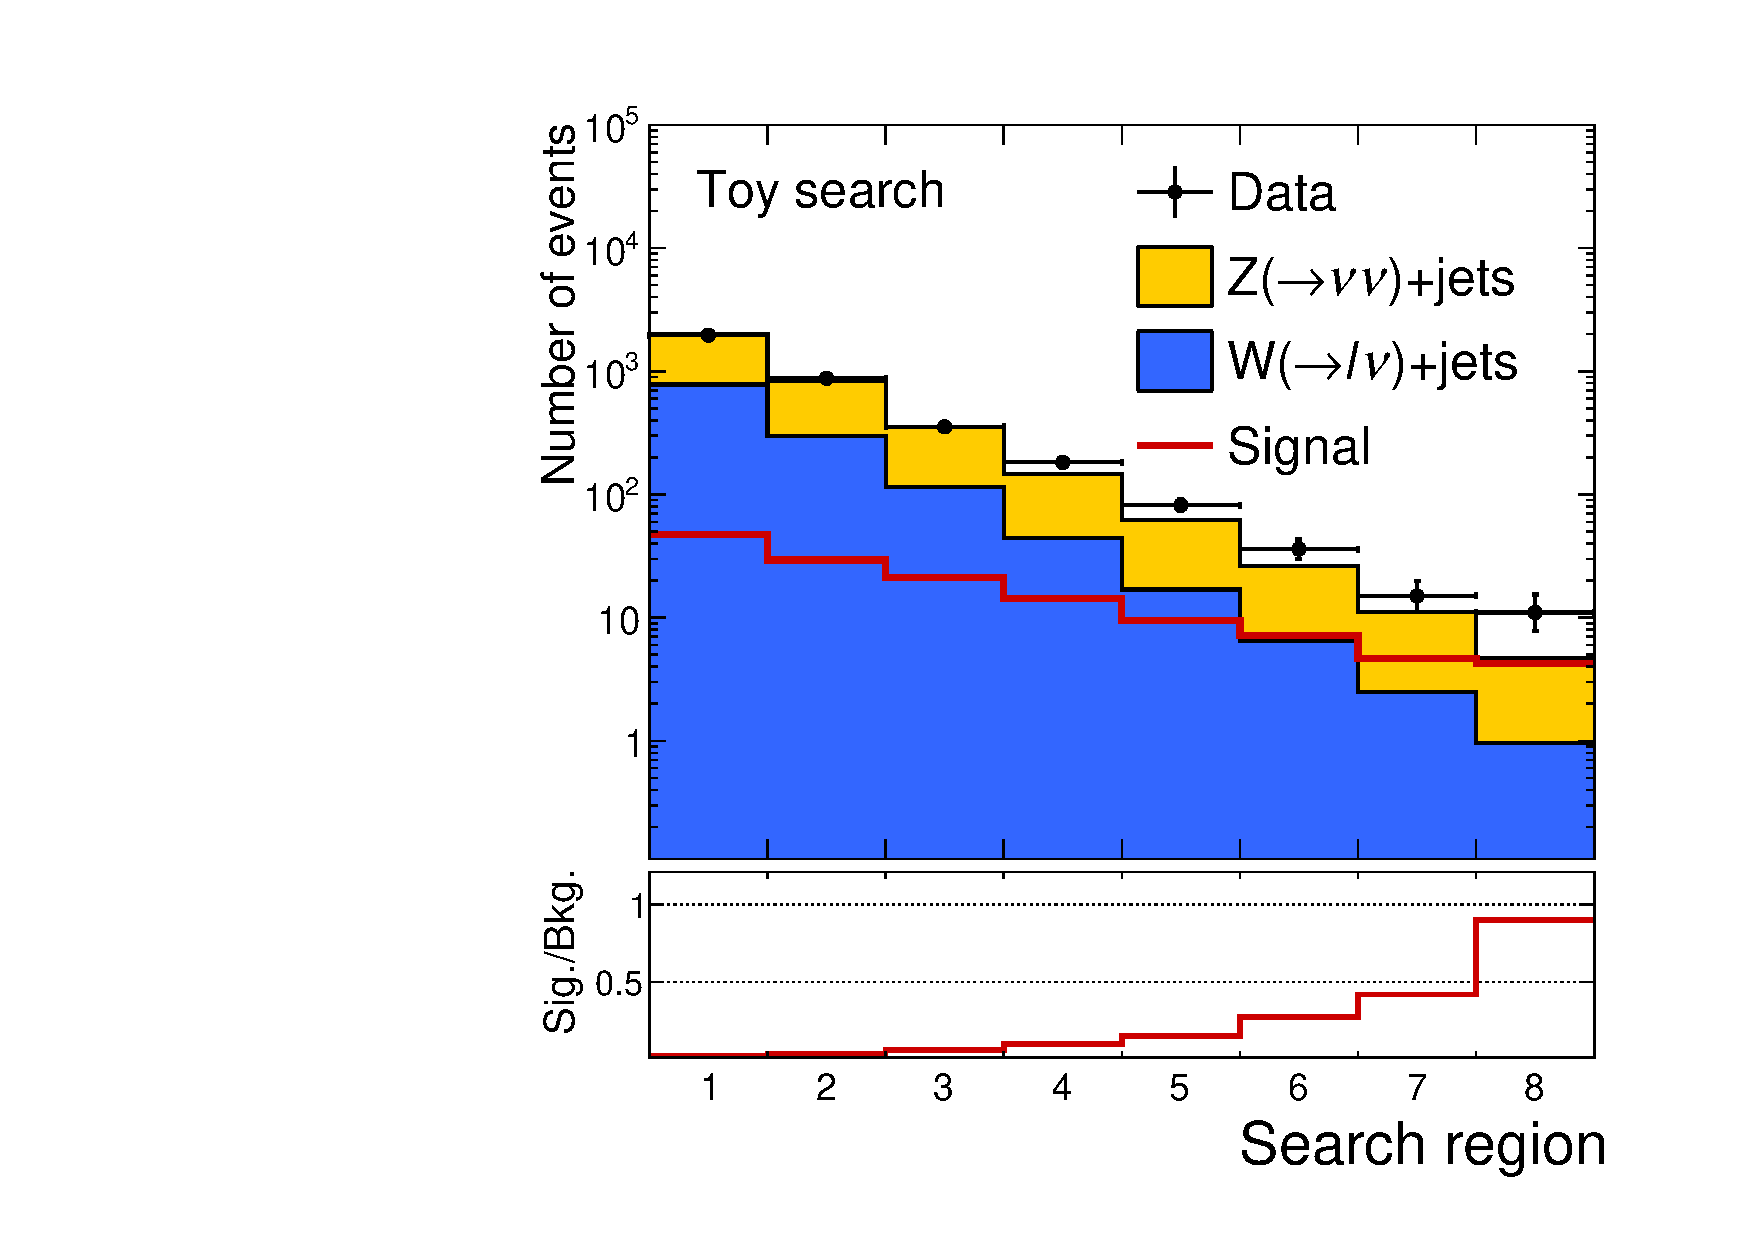
\includegraphics[width=1.2\cmsFigWidth]{figures/plot_dummy.pdf}}
   \subfloat[][]{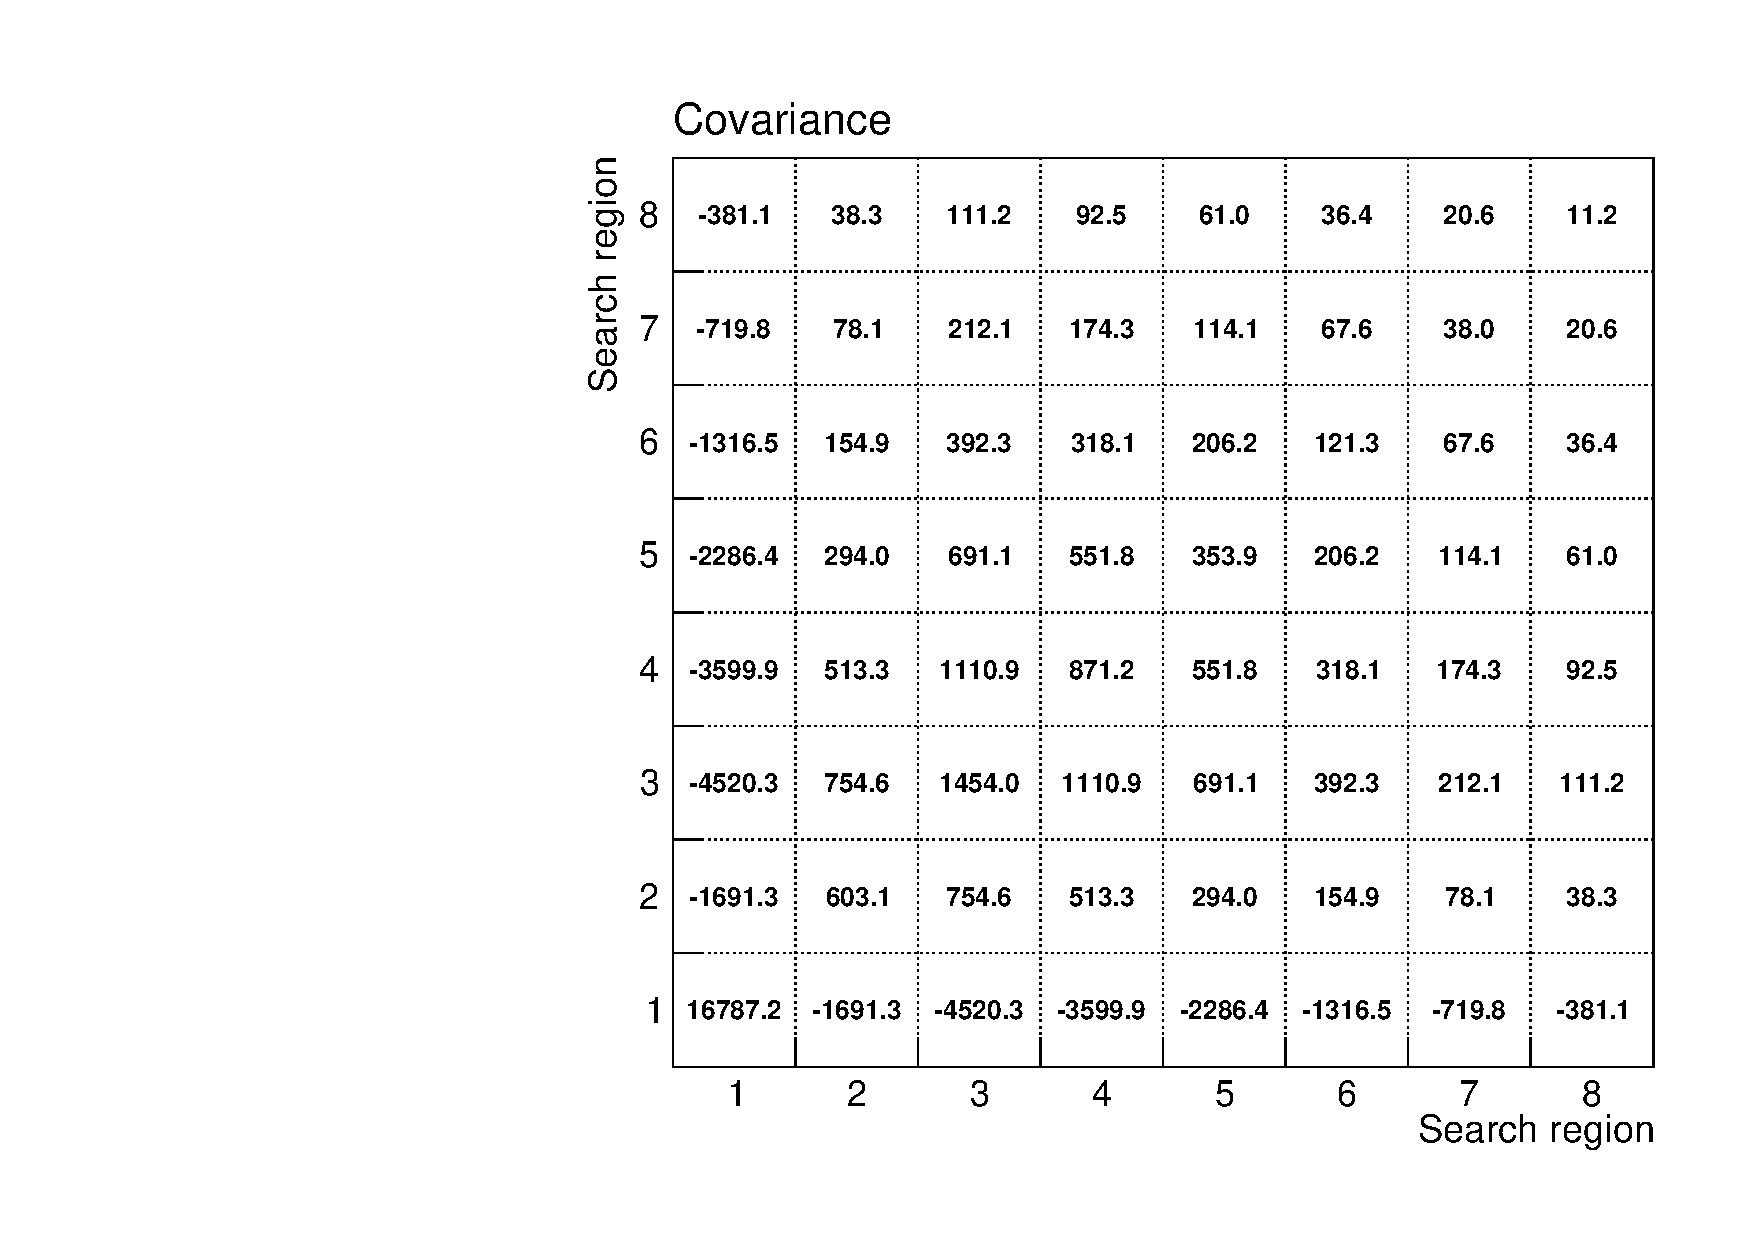
\includegraphics[width=1.2\cmsFigWidth]{figures/htsearch_covariance.pdf}}
   \caption{(a) Number of data, expected background and expected signal in the 8 search regions. The lower panel shows the ratio of the data to the total expected background. 
The shaded bands represent the uncertainty in the background contributions. (b) Covariance between the number of expected background events in each of the 8 search regions.}
   \label{fig:toy-example} 
  \end{center}
\end{figure}

The background estimates include systematic uncertainties related to theoretical uncertainties, when the backgrounds are derived using 
simulation, and experimental uncertainties related to the resolutions and response of the detector. They can also include a statistical component 
due to limited sample sizes of events in control regions used to estimate the backgrounds. Figure~\ref{} (b) gives the covariance between the total number of 
background events expected in each of the search regions. The non-zero off-diagonal values are a result of the fact that the estimate of the 
backgrounds are not independant in each bin. 

The information provided in Figure~\ref{fig:toy-example} is all that is necessary to reconstruct the likelihood in Equation~\ref{eq:full-likelihood} and 
can be summarised as follows; 

\begin{itemize}
\item {The number of observed events in each search region, $n_{i}$.}
\item {The background and signal expectations in each search region, $b_{i}$ and $s_{i}$.}
\item {The covariance between the number of background events in search region, $\mathrm{\mathbf{V}}=\left\{V_{ij}\right\}_{i,j=1}^{N}$. }
\end{itemize}

It is important to note that the estimates of both the background contributions and the 
covariance matrix do not use the data in the 8 search regions, making them statistically independant from the data. The data in the search regions 
can be used to further constrain the background (meaning to reduce the uncertainties on the nuisance parameters $\boldsymbol{\theta}$) through the use 
of the profiled likelihood ratio, which is defined as 

\begin{equation}
q(\mu) = -2\ln \dfrac {\mathcal{L}(\mu,\hat{\boldsymbol{\theta}}_{\mu})} {\mathcal{L}(\hat{\mu},\hat{\hat{\boldsymbol{\theta}}})}
\label{eq:llr}
\end{equation}

where $\hat{\mu}$ and $\hat{\hat{\boldsymbol{\theta}}}$ are the values of the parameters $\mu$ and $\boldsymbol{\theta}$ respectively, 
which maximise the likelihood. The values $\hat{\boldsymbol{\theta}}_{\mu}$ are the values of $\boldsymbol{\theta}$ which maximise the 
likelihood for a fixed value of $\mu$. 

The profiled likelihood is a common tool when defining test statistics for setting limits and quantifying excesses 
in BSM searches performed by the CMS collaboration, a full description of which  can be found in Refs.~\cite{}.

% covariance must be taken as the result of a maximum likelihood fit considering the control regions only. 
% If the control region is not included then the results fit may be taken. 
%%____________________________________________________________________________||
% \subsection{Motivation}
% \begin{itemize}
% \item Even with SSR recasters have insufficient information to reproduce analysis
% \item Full likelihood is overkill - what is necessary?
% \end{itemize}
% \subsection{Theory}
% \label{sec:sl-theory}
% \begin{itemize}
% \item Definition of simplified likelihood
% \item Inputs needed
% \item What's simplified? No signal systs, no CR, gaussian unc
% \end{itemize}
% \subsection{Procedure}
% \label{sec:sl-procedure}
% \begin{itemize}
% \item Determining correlation matrix
% \item Defining likelihood
% \item For study of impact setting off-diag elements to 0
% \end{itemize}
% \subsection{Signal contamination}
% \label{sec:signal-contamination}
% \begin{itemize}
% \item Definition of reduced efficiency method
% \item What do recasters need to take account of contamination?
% \end{itemize}
% \subsection{Results}
% \begin{itemize}
% \item Covariance matrix
% \item DeltaNLL vs r for example model (compare with + without correlations)
% \item Limit planes for several models (T1qqqq, T2tt, T2bb)
% \item Ratios + comparison to full
% \end{itemize}

%%____________________________________________________________________________||
\section{Aggregate search regions}
\label{sec:aggregate-signal-regions}

Inclusive searches for new physics typically use fine categorisation to allow
sensitivity to a wide range of models. However, this can make the use
of the search for re-interpretation impractical. 
This section describes how this categorisation may be simplified without neglecting the correlation 
between the search regions by defining aggregate search regions.

Considering the simplified likelihood defined in Equation~\ref{eq:full-likelihood},
the likelihood for aggregate search regions may be written by substituting the 
background predictions by,

\begin{align}
b_{i} + \theta_i \rightarrow b_I + \theta_I \equiv \sum_{i}(b_{i}) + \theta_I
\label{eq:b-agg}
\end{align}

where the sum is over all search regions being aggregated into search region $I$.
Note that the number of aggregate search regions must be fewer than the total number of search regions and 
every search region must be contained in a single aggregate search region. 
Similarly, the signal expectations and observed number of events are substituted by, 

\begin{align}
 s_{i}  \rightarrow s_{I} \equiv \sum_{i}s_{i},  &&  n_{i}  \rightarrow n_{I} \equiv \sum_{i}n_{i} 
\label{eq:b-agg}
\end{align}


The covariance matrix in the aggregate search regions is related to the full covariance matrix as, 

\begin{align}
V_{IJ}=\sum_{ij}V_{ij}
\label{eq:agg-cov}
\end{align}

where the sum is over all search regions being aggregated into search regions $I,J$.  The use of the simplified likelihood 
for the aggregated search regions relies on the same conditions outlined in Section~\ref{sec:simplified-likelihood}. 

\subsection{Example of the use of aggregate search regions}
\label{sec:agg-toy}

The same toy search described in Section~\ref{sec:sl-toy} is considered for use in an aggregated search. 
From Figure~\ref{fig:toy-example} it is clear that search regions 7 and 8  provide the dominant contribution to 
the sensitivity of the search as the ratio of the expected signal to the background is the largest in these two regions. 
One may therefore expect that search regions 1--6 can be neglected when deriving constraints on this particular BSM model. 
However, as the background expectations in these search regions are correlated with those in search regions 7 and 8, neglecting search regions 1--6 
will result in a loss of sensitivity.  
Alternatively, the search regions 1--6 may be aggregated using the covariance matrix shown in 
Figure~\ref{fig:covariance} and Equation~\ref{eq:agg-cov}. The resulting covariance
between the aggregate search regions is shown in Figure~\ref{fig:agg-covariance}.

\begin{figure}[hbt]
  \begin{center} 
   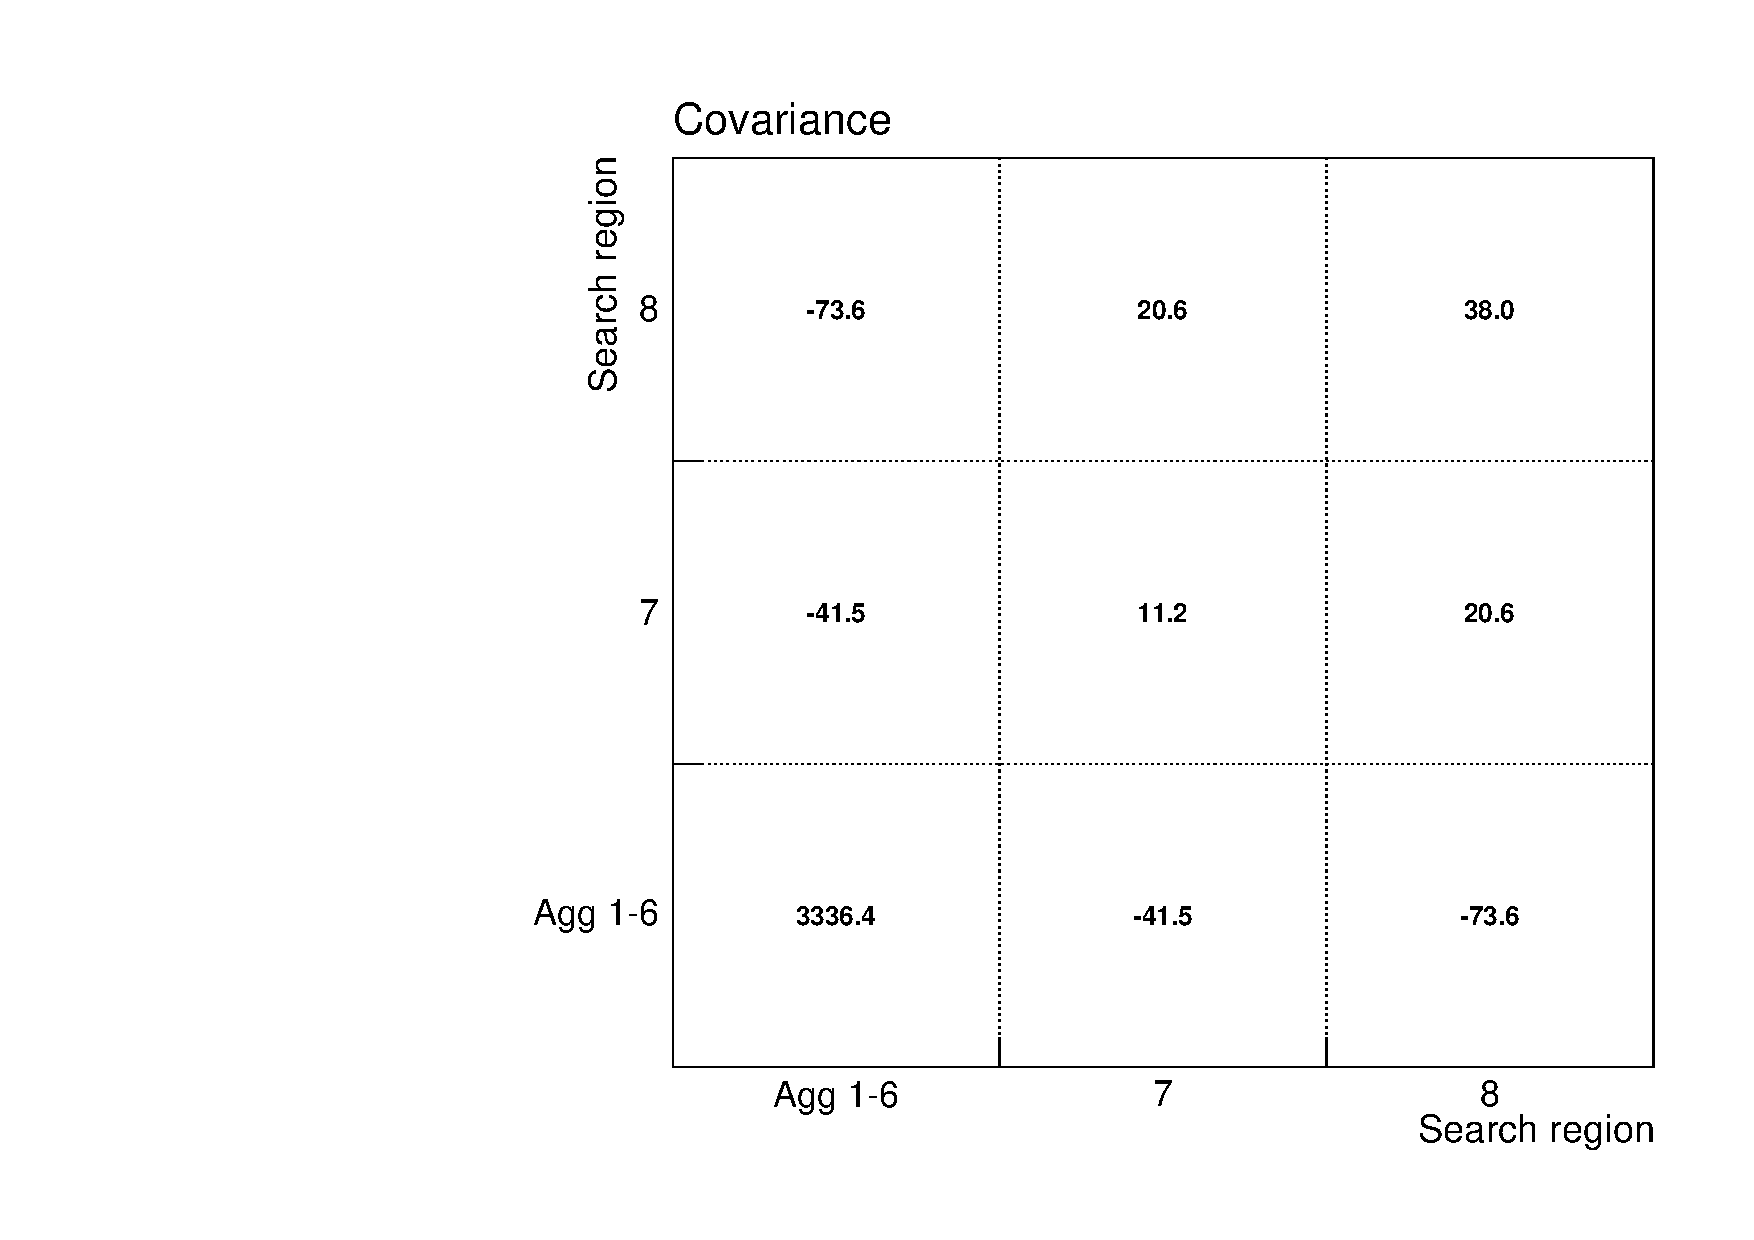
\includegraphics[width=1.5\cmsFigWidth]{figures/agg_htsearch_covariance.pdf}
   \caption{Covariance between the total rate of background contributions expected in each of the aggregated search regions}
   \label{fig:agg-covariance} 
  \end{center}
\end{figure}

Figure~\ref{fig:agg-likelihoodscan} shows the value of $q(\mu)$ as a function of $\mu$. The values when $q(\mu)$ 
is defined using the likelihood of Equation~\ref{eq:full-likelihood} using all 8 search regions, the aggregated search 
regions described above, and considering search regions 7 and 8 only are shown. There is good agreement between the curves using the 
aggregated search regions and using all 8 search regions. Neglecting the search regions 1--6 causes a change in the value
of $\hat{\mu}$. In addition, the width of the likelihood curve when neglecting these search regions is considerably
larger, implying a larger uncertainty estimate on $\mu$ and therefore poorer sensitivity to the BSM signal. 
This can be expected from the loss of constraint on the nuisance parameters when search regions 1--6 are neglected. 
Generically, the impact of removing search regions will depend on the size of the systematic uncertainties and their correlations 
between the search regions used and those which are neglected.

\begin{figure}[hbt]
  \begin{center} 
   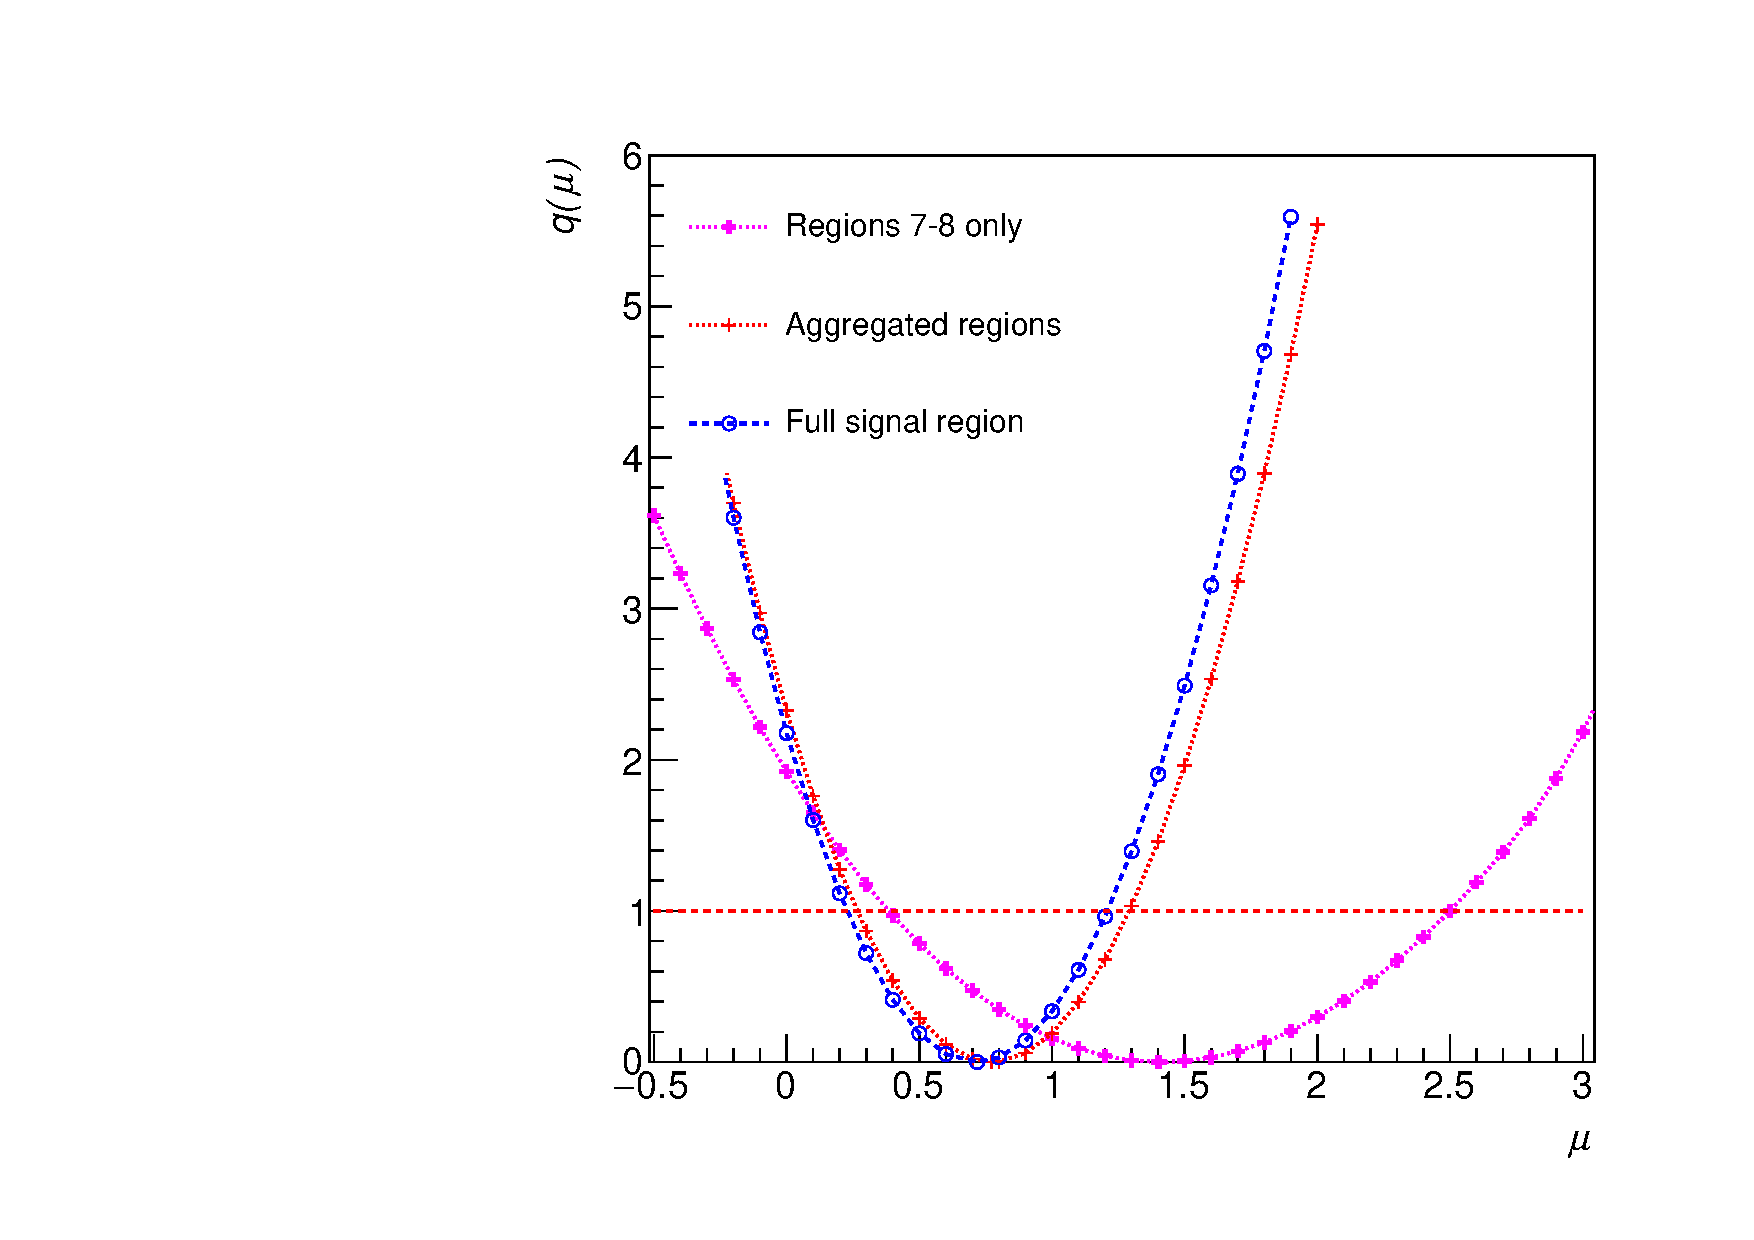
\includegraphics[width=1.5\cmsFigWidth]{figures/r_agg.pdf}
   \caption{The value of $q(\mu)$ defined using the simplified likelihood considering all 8 search regions (open blue points), the aggregated search regions (thin red crosses),
   and search regions 7 and 8 only (open magenta crosses).}
   \label{fig:agg-likelihoodscan} 
  \end{center}
\end{figure}

% %%____________________________________________________________________________||
\section{Highest excluding method}
\label{sec:high-exc-method}

A further simplification can be made from the simplified
likelihood defined in Section~\ref{sec:simplified-likelihood}.
Aggregate regions may be defined, which can be overlapping,
and the prediction and uncertainty for each of these regions
released. When deriving limits the recaster may define a
separate likelihood for each of these regions as shown in
Equation~\ref{eq-high-likelihood}.

\begin{equation}
\mathcal{L}_{i}=\mathrm{Pois}(n_{i} |\, b_{i} + s_{i}\times\mu)
\times\exp(\frac{(b_i-b_{i,0})^2}{\sigma_{ii}})
\label{eq:high-likelihood}
\end{equation}

where $sigma_{ii}$ is the variance for region $i$. When interpreting 
a model the recaster derives the 95\% upper limit for each of the 
regions separately and takes the exclusion from the bin 
giving the strongest limit for the model. The correlation
scheme does not need to be considered as only one region
provides the limit.

%%____________________________________________________________________________||
\section{Conclusions}
\label{sec:conclusions}
Searches for new physics by the CMS collaboration are performed using a wide variety of 
strategies and using events with different final states and kinematic properties. 
Re-interpreting these searches requires approximating the background model
and associated systematic uncertainties for the search. This can be 
achieved by definning a binned simplified likelihood where the systematic 
uncertainties on the backgrounds are approximated as correlated guassian constraints between the bins. 
To define the simplfied likelihood requires only the background predictions and covariance matrix which may be 
included in CMS publications. In addition, the number of search regions that must
be considered can be reduced, where necessary, through the use of aggregate regions. In summary, 
the use of the simplified likelihood allows a consistent and reliable approximation of the 
full likelihood used by CMS searches.



%%____________________________________________________________________________||

%%____________________________________________________________________________||
\bibliography{auto_generated}

%%____________________________________________________________________________||
 \appendix
\section{Appendices}

This section details validation of the use of simplified likelihoods in two example searches for BSM physics at CMS. 
\emph{The section is not intended for public dissemination and should be considered as internal material only.}

\subsection{Monojet/V search -- EXO-16-037}

The simplified likelihood approach has been validated in a search dark matter (DM) in  
13\TeV proton-proton collision events with a large missing transverse momentum and jets resulting from radiation 
of a gluon or a vector boson~\cite{}.

The search comprises two categories of events that are defined by the nature of the jets in the event. 
The first category, labelled mono-V, selects events which contain a ``fat-jet'' with a mass and substructure 
consistent with that of a hadrinically decaying W or Z boson. The second category, the monojet category, 
includes events failing the selection of the first but containing at least one high transverse momentum jet. 
In both categories, the magnitude of the missing transverse momentum ($\ETmiss$) is required to be greater than 200\GeV and 
each category is divided into several search regions defined as intervals in $\ETmiss$, 7 in the mono-V category and 22 in the 
monojet category making a total of 29 search regions.  The results of the search are interpreted 
in terms of simplified models for DM production~\cite{}, mediated via vector, axial vector, scalar or pseudoscalar interactions and 
in terms of a Higgs boson decaying to invisible particles. 

Figure~\ref{fig:monojetv} shows the number of events in each of the $\ETmiss$ intervals observed in each of two event 
categories as well as the total number of expected background events and the relative contribution of each source of background. The same information 
is tabulated in Tables~\ref{tab:monojettab} and~\ref{tab:monovtab}. 

\begin{figure}[hbt!]
  \begin{center} 
   \subfloat[][]{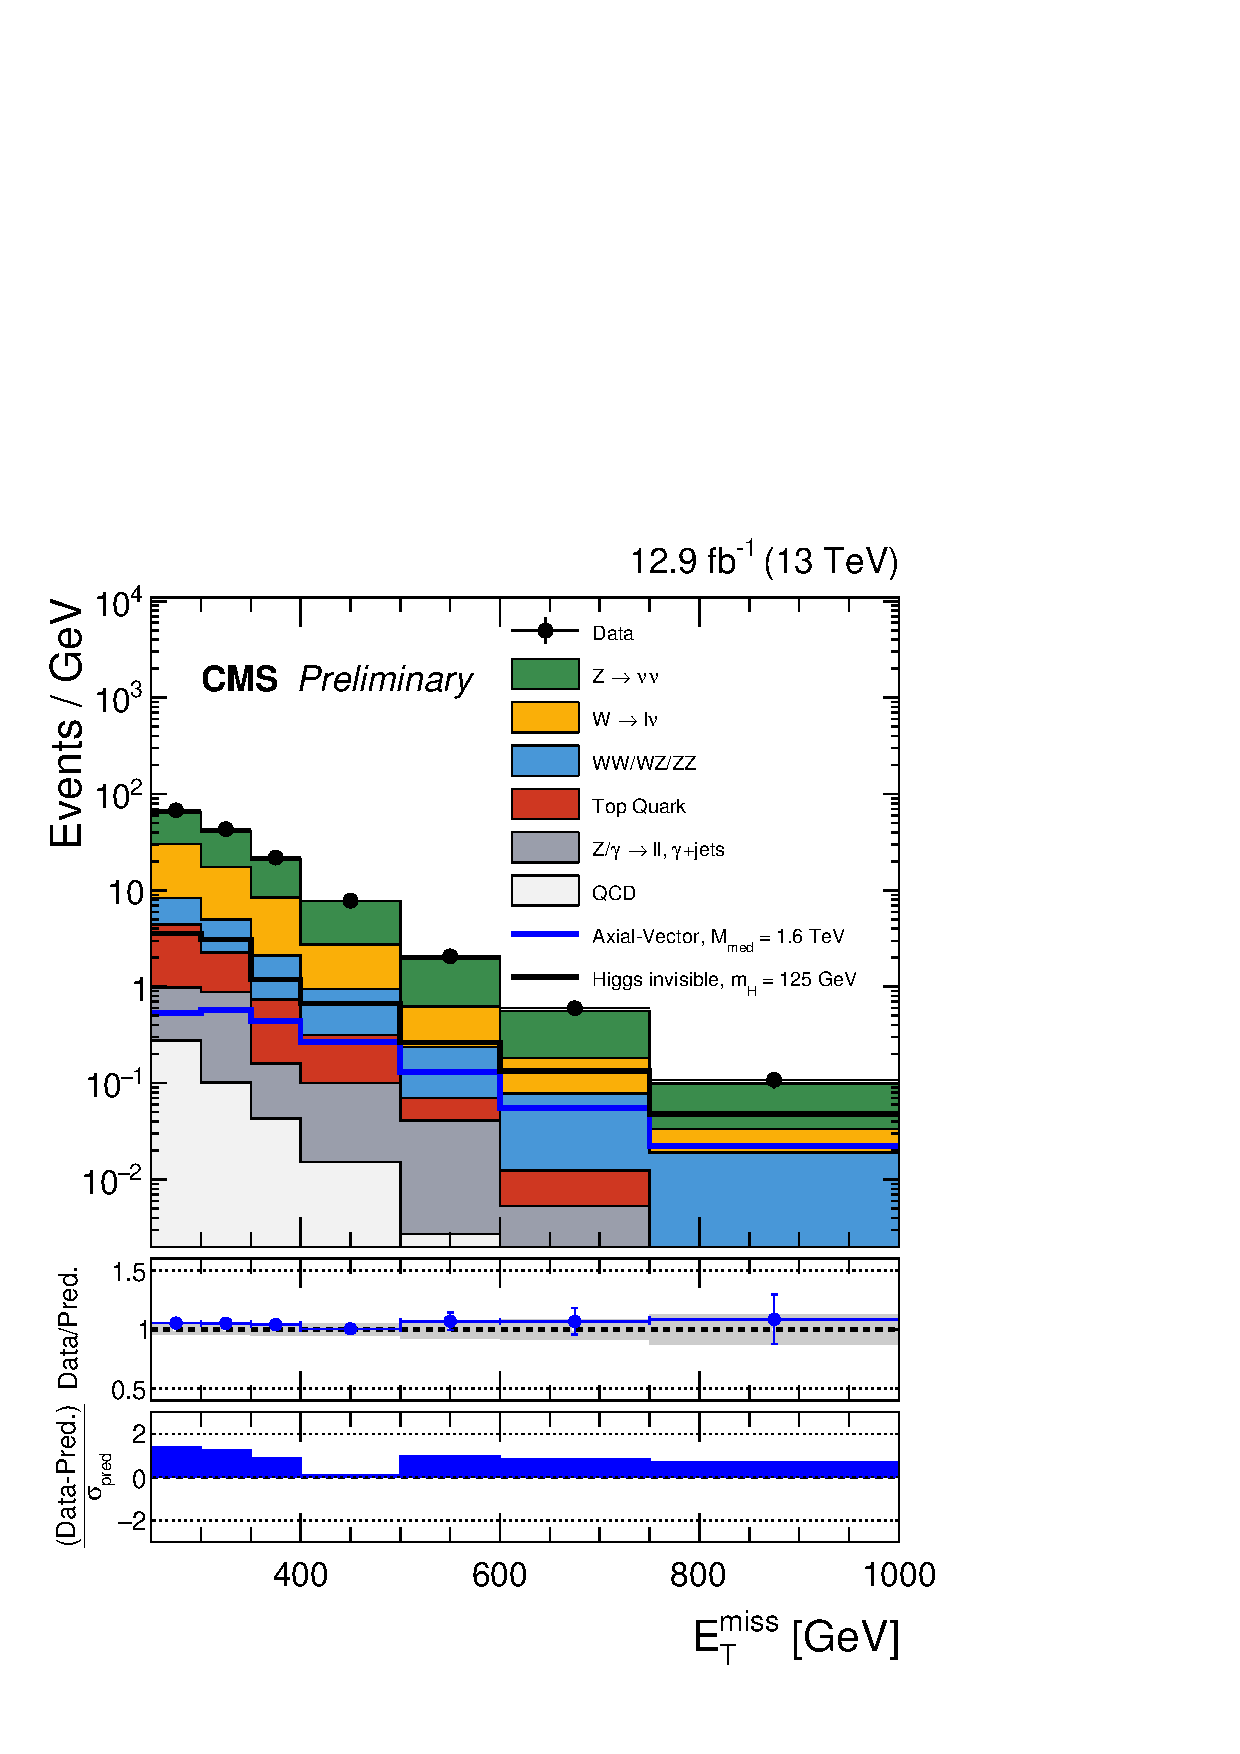
\includegraphics[width=1.2\cmsFigWidth]{figures/postfit_sig_MV_SRmask.pdf}}
   \subfloat[][]{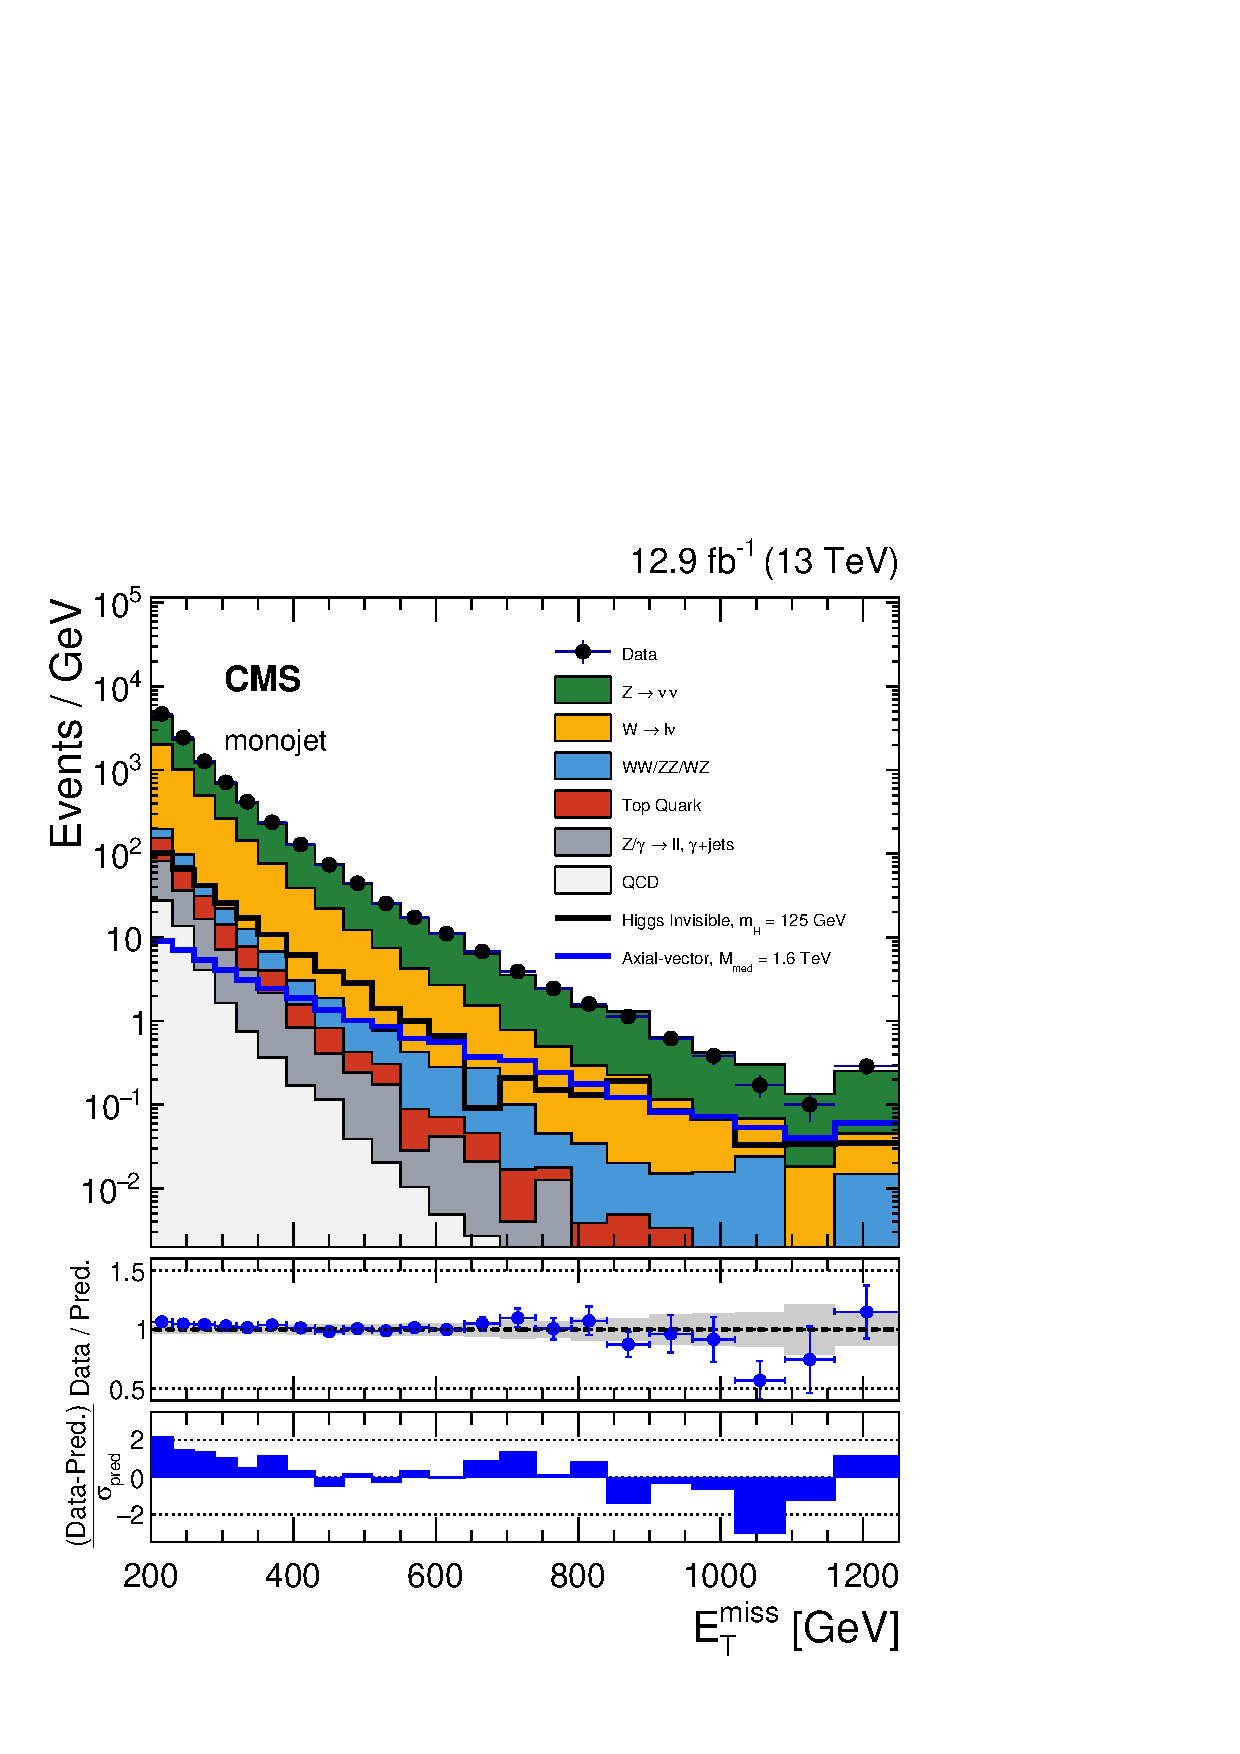
\includegraphics[width=1.2\cmsFigWidth]{figures/monojet_PULLS_MASKED_prefit_postfit_signal.pdf}}
\caption{
      Observed number of events in each \ETmiss interval in the (a) mono-V and (b) monojet categories compared with the background expectations for various SM processes.
      The last bin includes all events with \ETmiss$ > 1160 \GeV$ for the monojet category and \ETm$ > 750 \GeV$ for the mono-V category.
      The expected background distributions are evaluated after performing a combined fit to the data in all the control regions, but not including the search regions.
      Expected signal distributions from the 125 GeV Higgs boson decaying exclusively to invisible particles, and a 1.6 TeV axial-vector mediator decaying to 1 GeV DM particles, are overlaid.
      The ratio of data with the background prediction is shown for both the monojet and mono-V signal regions.
      The gray bands in these ratio plots indicate the uncertainty in the background prediction and are dervied as the square root of the variance of the expected number of background events.
      Finally the difference between data and the background prediction relative to the uncertainty in the prediction,
      are also shown in the lower panels.
   }
   \label{fig:monojetv} 
  \end{center}
\end{figure}


\begin{table}[!htb]
\caption{Observed and expected event yields in each \ETmiss search region for various background processes in the mono-V category. The background yields and the
         corresponding uncertainties are obtained after performing a combined fit to data in all the control regions and do not use data in any of the search regions.
	 }
 \begin{center}
 \scriptsize
 \begin{tabular}{c|c|c|c|c|c|c|c}
 \hline
 \ETMiss (GeV) & Data & $\mathrm{Z} \rightarrow \nu\nu$ & $\mathrm{W} \rightarrow \ell\nu$ & Top quark & Dibosons & Other & Total Bkg. \\
 \hline
250--300 & 3395 & 1700 $\pm$ 88  & 1100  $\pm$ 65  & 171 $\pm$ 24   & 195 $\pm$ 35    & 49.4 $\pm$ 10.8 & 3220 $\pm$ 130 \\
300--350 & 2162 & 1180 $\pm$ 68  & 627   $\pm$ 37  & 68.8 $\pm$ 9.7 & 135 $\pm$ 24    & 44.2 $\pm$ 7.2  & 2050 $\pm$ 88 \\
350--400 & 1093 & 629 $\pm$ 37   & 314   $\pm$ 21  & 28.9 $\pm$ 4.1 & 68.5 $\pm$ 12   & 8.0 $\pm$ 1.8   & 1048 $\pm$ 51 \\
400--500 & 780  & 500 $\pm$ 33   & 181   $\pm$ 13  & 21.4 $\pm$ 3.0 & 62.8 $\pm$ 11   & 10.1 $\pm$ 1.8  & 775  $\pm$ 40 \\
500--600 & 207  & 131 $\pm$ 12   & 38.5  $\pm$ 3.4 & 2.9 $\pm$ 0.4  & 16.8 $\pm$ 3.0  & 4.1 $\pm$ 0.8   & 193  $\pm$ 14 \\
600--750 & 90   & 57.1 $\pm$ 5.9 & 15.6 $\pm$ 1.6  & 1.0 $\pm$ 0.1  & 9.8 $\pm$ 1.7   & 0.8 $\pm$ 0.1   & 84.2 $\pm$ 6.9 \\
750--1000 & 27  & 16.5 $\pm$ 2.7 & 3.6  $\pm$ 0.6  & -              & 4.7 $\pm$ 0.8   & 0.01 $\pm$ 0.01 & 24.8 $\pm$ 3.1 \\
 \hline
\end{tabular}
\end{center}
\label{tab:monovtab}
\end{table}



\begin{table}[htb]
\caption{Observed and expected event yields in each \ETmiss search region for various background processes in the monojet category. The background yields and the
         corresponding uncertainties are obtained after performing a combined fit to data in all the control regions and do not use data in any of the search regions.
	 }
 \begin{center}
 \scriptsize
 \begin{tabular}{c|c|c|c|c|c|c|c}
 \hline
 \ETmiss (GeV) & Data & $\mathrm{Z} \rightarrow \nu\nu$ & $\mathrm{W} \rightarrow \ell\nu$ & Top quark & Dibosons & Other & Total Bkg. \\
 \hline
200--230 & 140642 & 71300 $\pm$ 2200 & 54600 $\pm$ 2300 & 2140 $\pm$ 320  & 1320 $\pm$ 220   & 2470 $\pm$ 310   & 132100 $\pm$ 4000 \\
230--260 & 73114  & 39500 $\pm$ 1300 & 27500 $\pm$ 1200 & 1060 $\pm$ 160  & 790 $\pm$ 130    & 1090 $\pm$ 130   & 69900  $\pm$ 2200 \\
260--290 & 38321  & 21900 $\pm$ 670  & 13600 $\pm$ 550  & 440 $\pm$ 65    & 364 $\pm$ 61     & 498 $\pm$  65    & 36800  $\pm$ 1100 \\
290--320 & 21417  & 12900 $\pm$ 400  & 7300 $\pm$ 290   & 210 $\pm$ 31    & 235 $\pm$ 40     & 216 $\pm$ 30     & 20780  $\pm$ 630 \\
320--350 & 12525  & 8000 $\pm$ 280   & 4000 $\pm$ 170   & 107 $\pm$ 16    & 145 $\pm$ 24     & 124 $\pm$ 18     & 12340 $\pm$ 400 \\
350--390 & 9515   & 6100 $\pm$ 220   & 2800 $\pm$ 130   & 74  $\pm$ 11    & 111 $\pm$ 19     & 87  $\pm$ 13     & 9160 $\pm$ 320 \\
390--430 & 5174   & 3500 $\pm$ 160   & 1434 $\pm$ 66    & 30.1 $\pm$ 4.5  & 58.4 $\pm$ 9.9   & 33.4 $\pm$ 5.3   & 5100 $\pm$ 200 \\
430--470 & 2947   & 2100 $\pm$ 98    & 816 $\pm$ 37     & 16.6 $\pm$ 2.5  & 42.4 $\pm$ 7.1   & 16.3 $\pm$ 2.7   & 3000 $\pm$ 120 \\
470--510 & 1777   & 1300 $\pm$ 66    & 450 $\pm$ 20     & 7.4 $\pm$ 1.1   & 24.6 $\pm$ 4.1   & 9.6 $\pm$ 1.6    & 1763 $\pm$ 79 \\
510--550 & 1021   & 735 $\pm$ 39     & 266 $\pm$ 13     & 5.2 $\pm$ 0.8   & 18.5 $\pm$ 3.1   & 7.0 $\pm$ 1.3    & 1032 $\pm$ 48 \\
550--590 & 694    & 513 $\pm$ 31     & 152 $\pm$ 8      & 2.4 $\pm$ 0.4   & 13.5 $\pm$ 2.3   & 1.1 $\pm$ 0.3    & 683 $\pm$ 37 \\
590--640 & 554    & 419 $\pm$ 23     & 120 $\pm$ 6      & 1.5 $\pm$ 0.2   & 10.6 $\pm$ 1.8   & 2.1 $\pm$ 0.4    & 554 $\pm$ 28 \\
640--690 & 339    & 246 $\pm$ 16     & 62.8 $\pm$ 3.8   & 1.3 $\pm$ 0.2   & 11.4 $\pm$ 1.9   & 1.0 $\pm$ 0.2    & 322 $\pm$ 19 \\
690--740 & 196    & 139 $\pm$ 11     & 34.2 $\pm$ 2.4   & 0.6 $\pm$ 0.1   & 4.2 $\pm$ 0.7    & 0.20 $\pm$ 0.07  & 178 $\pm$ 13 \\
740--790 & 123    & 97.2 $\pm$ 7.2   & 22.7 $\pm$ 1.7   & 0.22 $\pm$ 0.03 & 1.4 $\pm$ 0.2    & 0.63 $\pm$ 0.12  & 122 $\pm$ 8 \\
790--840 & 80     & 59.8 $\pm$ 5.8   & 12.9 $\pm$ 1.2   & 0.13 $\pm$ 0.02 & 1.5 $\pm$ 0.3    & 0.05 $\pm$ 0.02  & 74.5 $\pm$ 6.6 \\
840--900 & 68     & 64.3 $\pm$ 6.4   & 12.3 $\pm$ 1.1   & 0.24 $\pm$ 0.04 & 0.92 $\pm$ 0.11  & 0.03 $\pm$ 0.01  & 77.8 $\pm$ 7.2 \\
900--960 & 37     & 31.5 $\pm$ 4.3   & 6.0 $\pm$ 0.7    & 0.21 $\pm$ 0.03 & 0.74 $\pm$ 0.10  & 0.01 $\pm$ 0.01  & 38.4 $\pm$ 4.8 \\
960--1020 & 23    & 20.8 $\pm$ 3.0   & 3.4 $\pm$ 0.5    & -               & 0.94 $\pm$ 0.23  & 0.01 $\pm$ 0.01  & 25.1 $\pm$ 3.4 \\
1020--1090 & 12   & 16.3 $\pm$ 2.6   & 3.1 $\pm$ 0.5    & 0.04 $\pm$ 0.01 & 1.6  $\pm$ 0.3   & 0.01 $\pm$ 0.01  & 21.1 $\pm$ 3.0 \\
1090--1160 & 7    & 8.1 $\pm$ 1.8    & 1.3 $\pm$ 0.3    & -               & -                & -                & 9.4 $\pm$ 1.9 \\
1160--1250 & 26   & 18.6 $\pm$ 2.7   & 2.7 $\pm$ 0.4    & -               & 1.3 $\pm$ 0.2    & -                & 22.6 $\pm$ 3.0 \\
 \hline
\end{tabular}
\end{center}
\label{tab:monojettab}
\end{table}


The dominant backgrounds in this search are derived by defining several control regions in the data and simultaneously fitting for their contribution 
in the control and search regions. The full procedure is described in detail in Secion 4 of Ref.~\ref{}. The smaller backgrounds are estimated from 
simulation, tuned using data. The full likelihood model used in this search contains $\mathcal{O}(100)$ nuisance parameters relating to theoretical 
extrapolations between the control regions and the search regions as well as experimental sytematic uncertainties on 
the lepton identification and jet reconstruction used. The full likelihood is therefore prohibitavely complicated, making its publication unfeasible. 
Instead, the simplified likelihood approach can be used. Figure~\ref{fig:fullcovariance} shows the correlation coefficeints, \left\{$\rho_{ij}\right\}_{i,j=1}^{29}$, between the total background 
rate in each of the 29 search regions. Both the correlations and the total expected background contributions are dervied without using the data in the 
search regions, allowing for construction of the simplified likelihood. Note that covariance matrix can be derived from the correlation coefficients and 
the variance (the square of the last colum in Tables~\ref{tab:monojettab} and~\ref{tab:monovtab}) since, 

\begin{align}
V_{ij} = \rho_{ij}\cdot\sigma_{i}\sigma_{j}, &&  \sigma_{k}^{2}=V_{kk}
\end{align}



%%____________________________________________________________________________||
\subsection{Validation with the \alphat analysis}
The \alphat analysis is an inclusive search for supersymmetry which
uses a fine categorisation in \nj,\nb,\scalht,and \mht to provide
sensitivity to a wide range of new physics models. The results 
of this search using 12.9\fb of data at 13\TeV from Run 2 of the LHC
are described fully in \cite{CMS-PAS-SUS-16-016}. In this section,
the use of aggregate regions is discribed for the \alphat analysis, as well as a 
validation of the simplified likelihood method.

\subsubsection{Defining agregate regions}

The \alphat analysis is a binned analysis which uses one or more signal depleted control region(s) 
to constrain standard model backgrounds in the signal region with relevant systematics.
The likelihood may be written in two parts, splitting the signal and control regions. 
To illustrate how the aggregate regions may be defined from the full likelihood, 
a simplified scenario is considerd in which each signal bin contains one background, however,
it is easy to see how this may be extended. In this case, the signal region section of the likehood may be written
as a product over bins, i, as in Equation~\ref{eq:hadronicLikelihood}.

\begin{equation}
\mathcal{L}_{\mathrm{signal}}=\prod_i{\mathrm{Pois}(n_{\mathrm{signal},i} |\, b_{\mathrm{signal},i}
\times\overline{\rho}_{\mathrm{signal},i}\times{a_i} + s_{\mathrm{signal}}\times\overline{\rho}^\mathrm{s}_{\mathrm{signal},i}\times\mu)}
\label{eq:hadronicLikelihood}
\end{equation}

where $n_{\mathrm{signal},i}$ is the observation in the signal bin, $b_{\mathrm{signal},i}$
the background prediction from simulation, $\overline{\rho_{i}}$ the set of systematics
on the signal region prediction, ${a_i}$ an unconstrained parameter that will connect to the 
control region, $s_{\mathrm{sig}}$ the signal model contribution from simulation, 
$\overline{\rho}_{i,sig}$ the set of systematics on the signal contribution and $\mu$ the
unconstrained signal strength parameter.  The connection to each control region 
may be written as in Equation~\ref{eq:controlLikelihood}.

\begin{equation}
\mathcal{L}_{\mathrm{control},i}=\prod_i{\mathrm{Pois}(n_{\mathrm{control},i} |\, b_{\mathrm{control},i}
\times\overline{\rho}_{\mathrm{control}}\times{a_i} + s_{\mathrm{control}}\times\overline{\rho}^\mathrm{s}_{\mathrm{control},i}\times\mu)}
\label{eq:controlLikelihood}
\end{equation}

where parameters are as defined in Equation~\ref{eq:hadronicLikelihood} but for the control region. 
Here $\overline{\rho}_{\mathrm{control},i}$ contains both systematic uncertainties on the control region
and on the connection of the control to signal region. Correlation between bins in the signal
and control regions are introduced through the correlation or anticorrelation of the systematic uncertainties
contained in both $\overline{\rho}_{\mathrm{signal},i}$ and $\overline{\rho}_{\mathrm{control},i}$. Additional correlations are introduced if
control regions are used to predict the background in multiple signal region bins. 
The overall likelihood of $\mathcal{L} = \mathcal{L}_{\mathrm{signal}}\times\mathcal{L}_{\mathrm{control}}$
is then minimized with respect to $\mu$,$\rho$ and $\rho_^{mathrm{s}}$. 

From $\mathcal{L}$ the likelihood for the aggregate regions may then be defined as in Equation~\ref{eq:agg-hadronicLikelihood}.

\begin{equation}
\mathcal{L}_{\mathrm{l}}=\prod_{agg}{\mathrm{Pois}(n_{\mathrm{signal},agg} |\,\sum_i^{k_{agg}}{b_{\mathrm{signal},i}
\times\overline{\rho}_{\mathrm{signal},i}\times{a_i} + s_{\mathrm{signal}}\times\overline{\rho}^\mathrm{s}_{\mathrm{signal},i}\times\mu)}}
\times\mathcal{L}_{\mathrm{control}}$
\label{eq:agg-hadronicLikelihood}
\end{equation}

where the contributions of all bins being merged into aggregate regions are 
summed to provide a total background and signal contribution to the aggregate bin. 
The control region section of the likelihood is unchanged and so the correlation model 
for the predictions is maintained. The likelihood is minimized with respect to $mu$,$\rho$, $\a_i$, $\rho_^{mathrm{s}}$ as 
before. For analyses which do not include a control region explicitely in the likelihood 
the aggregation process is similar, however, in this case the parameters $a_i$ are not 
freely floating but are instead constrained according to a pdf, such as a gamma distribution, 
which encodes the uncertainty from the control region. The form of the nominal and aggregate
likelihoods are otherwise unchanged. In Section~\ref{sec:ssr-alphat} an example of the use of 
aggregate regions is shown for the \alphat analysis.

\subsubsection{Application of the the aggregate regions with the \alphat analysis}
\label{sec:ssr-alphat}
The final \nj,\nb categories and \scalht binning used for the full likelihood 
are summarised in Table~\ref{tab:binning}. These bins are further split into
$100 \GeV$ \mht bins as defined in \cite{alphaT}. The control region
predictions are inclusive in \mht but binned according to Table~\ref{tab:binning}.

\begin{table}[htb!]
  \topcaption{Summary of the lower bounds of the first and final bins
    in \scalht (the latter in parentheses) as a function of \njet and
    \nb. Intermediate \scalht bins are taken from 200,250,300,400,500,600,700,$>800\GeV$} 
  \label{tab:binning}
  \centering
  \footnotesize
  \begin{tabular}{ lrrrr }
    \hline
%    \njet                   & \multicolumn{4}{c}{\nb}                                           \\
%    \cline{2-5}
%                            & 0         & 1         & 2         & $\geq$3                       \\
    $\njet \backslash\, \nb$ & 0         & 1         & 2         & $\geq$3                       \\
    \hline
    \multicolumn{5}{l}{\bf Monojet}                                                              \\
    1                        & 200 (600) & 200 (500) & -     & -                         \\
    \multicolumn{5}{l}{\bf Asymmetric}                                                           \\
    2                        & 200 (600) & 200 (500) & 200 (400) & -                         \\
    3                        & 200 (600) & 200 (600) & 200 (500) & 200 (300)                     \\
    4                        & 200 (600) & 200 (600) & 200 (600) & 250 (400)                     \\
    $\geq$5                  & 250 (600) & 250 (600) & 250 (600) & 300 (500)                     \\
    \multicolumn{5}{l}{\bf Symmetric}                                                            \\
    2                        & 200 (800) & 200 (800) & 200 (600) & -                         \\
    3                        & 200 (800) & 250 (800) & 250 (800) & \phantom{0}-\phantom{0} (250) \\
    4                        & 300 (800) & 300 (800) & 300 (800) & 300 (800)                     \\
    $\geq$5                  & 350 (800) & 350 (800) & 350 (800) & 350 (800)                     \\
    \hline
  \end{tabular}
\end{table}

The $\mathcal{O}800$ bins provide generic sensitivity but are not optimal
for simple reinterpretation. A simplification can be made that maintains
sensitivity to a large class of models through the use of aggregate regions.
The thirty one jet categories are reduced to eight aggregate jet categories while
the up to eight \scalht bins are merged into one ($\scalht \geq 200 GeV$).
The final categories are shown in Table~\ref{tab:agg-binnning}.
These are defined to be disjoint, contiguous and to cover the full
signal region and so in combination to reflect sensitivity from the
full signal region phase space. In addition,
for each aggregate category eight exclusive \mht bins with
lower bounds $100,200,300,400,500,600,700,\ge800GeV$ are defined.

\begin{table}[tb]
  \topcaption{Aggregate region bins. The \scalht dimension is
  merged to $\geq200\GeV$, \nb to two categories of \nb = $0,1$ and $\geq2$. 
  The merged \nj~ categories are summarised in this table. Each category is
  further binned using eight \mht bins with lower bounds from $100-800\GeV$.}
  \label{tab:agg-binning}
  \centering
  \footnotesize
  \begin{tabular}{ llll }
    \hline
    \nj topology & \multicolumn{3}{l}{Merged jet categories} \\
    \hline
     & \bf Monojet & \bf Asymmetric& \bf Symmetric \\
    Monojet-like & 1 & 2 & 2                         \\
    Asymmetric high \nj& - & 3, 4, $\geq5$ & -                 \\
    Mid \nj & - &  3, 4 & -                        \\
    High \nj & - & $\geq5$ & -                     \\
    \hline
  \end{tabular}
\end{table}

The jet categories are merged to four seperate categories motivated by their sensitivity to 
different new physics topologies. For example, the Monojet-like topology is targeted towards
dark matter models and compressed spectra while the high \nj topology targets 
uncompressed gluino and squark models. The b-jet categories are combined 
as $\nb=0,1$ \nb models and $\nb\geq2$ targeted at
light and heavy flavour new physics respectively. Finally, the \scalht dimension is 
entirely merged as the \mht dimension generally provides better sensitivity
for new physics models. The use of the aggregate regions ensures 
that the backgrounds are still predicted by the nominal, finely binned regions (with appropriate systematics).

\subsubsection{Results using aggregate regions for the \alphat analysis}

The aggregate regions provide an easily comprehensible
overview of the signal region when compared to the results
of the nominal signal bins. Figure~\ref{fig:aggFitResult} shows
the post fit predictions in the mid and high \nj categories
for the aggregate regions compared to the observed data.

To evaluate the effect on the reach of the \alphat analysis the expected and observed 95\% upper limit
on the signal strength, defined as in \cite{limit-stuff}, for the full signal region 
is compared that using the aggregate regions. The limits are shown side by side
in Fig~\ref{fig:limit-planes} for three models, T2tt T2bb and T1bbbb. Where the mass
splittings are small the expected limits typically reduce by $\mathcal{O} 100\GeV$ 
compared to the full signal region.

The predictions from the aggregate regions can be used to provide predictions and uncertainties
to allow recasters to interpret their own models. In the case of the \alphat search
this is significantly easier than recasting the full signal region. To make best use of this information, 
as will be discussed in Section~\ref{sec:simplified-likelihood}, 
the covariance matrix encoding the level of correlation between bins must also be utilised.
\clearpage
\begin{figure}[!tbhp]
    \caption{ Signal region predictions and data observations for the aggregate regions. 
    The predictions are made using a fit to the control region only. \label{fig:aggFitResult} }
  \begin{center}
    \subfigure[Mid \nj, $\nb \leq 1$]   { 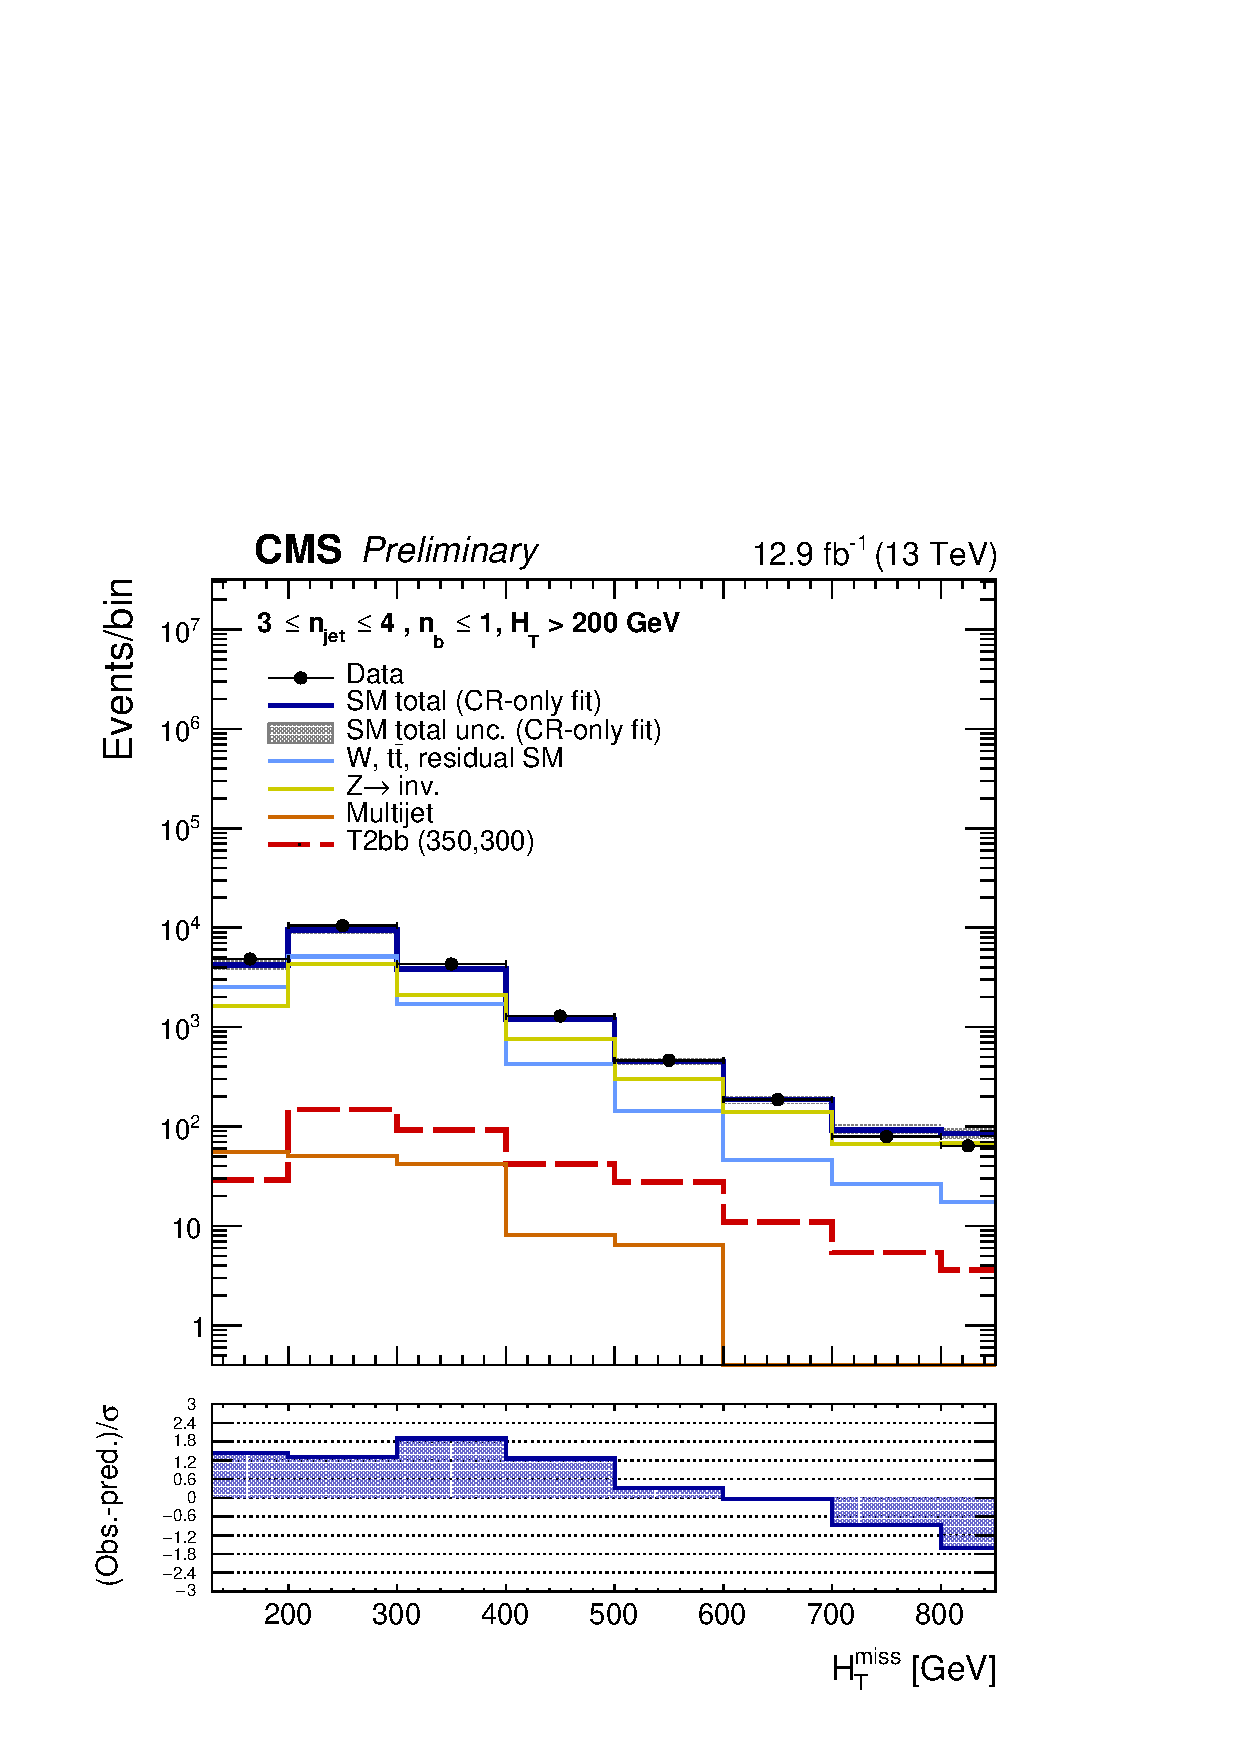
\includegraphics[width=0.4\textwidth]{figures/alphaT/agg_fitResults/mhtShape_le1b_ge3j_200_Inf_crfit_aux.pdf} } ~~
    \subfigure[Mid \nj, $\nb \geq 2$]{ 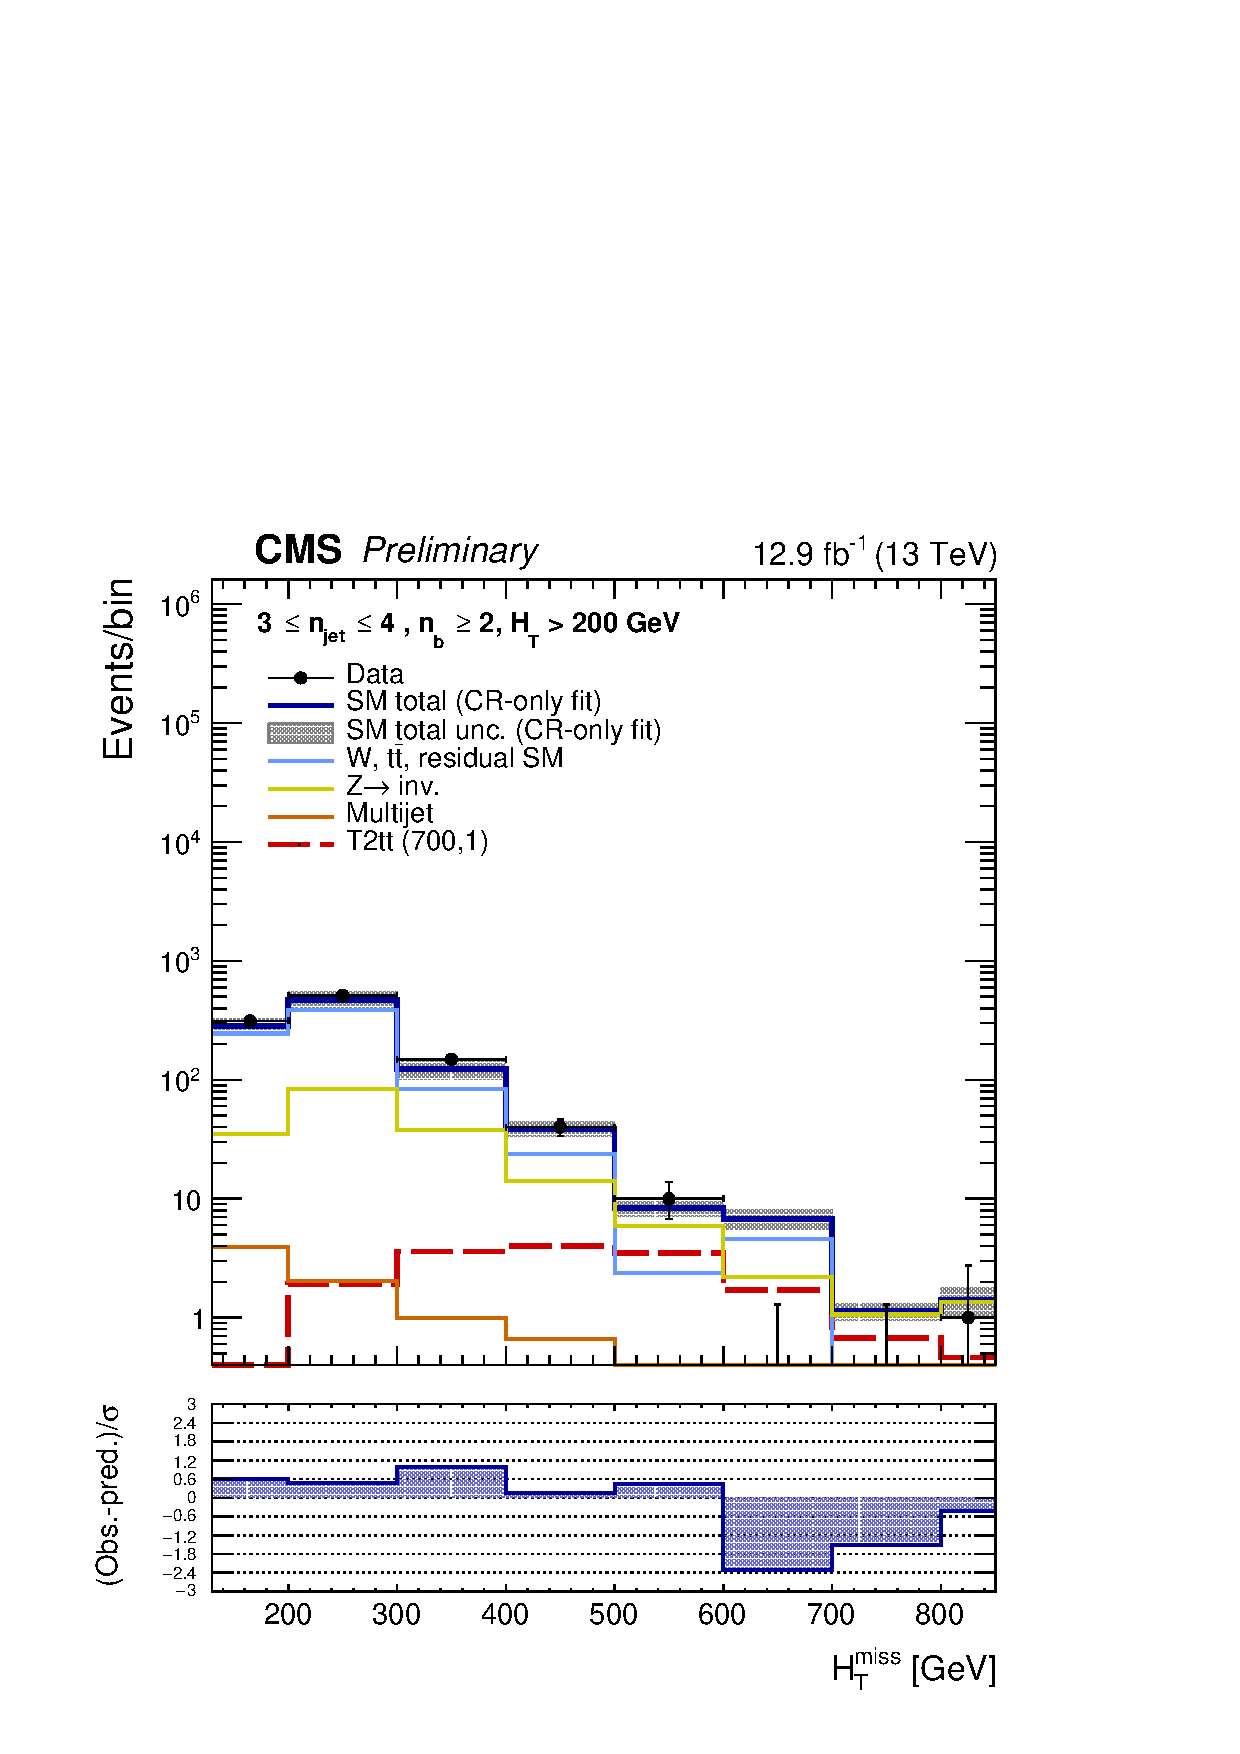
\includegraphics[width=0.4\textwidth]{figures/alphaT/agg_fitResults/mhtShape_ge2b_ge3j_200_Inf_crfit_aux.pdf} } \\
    \subfigure[High \nj, $\nb \leq 1$]   { 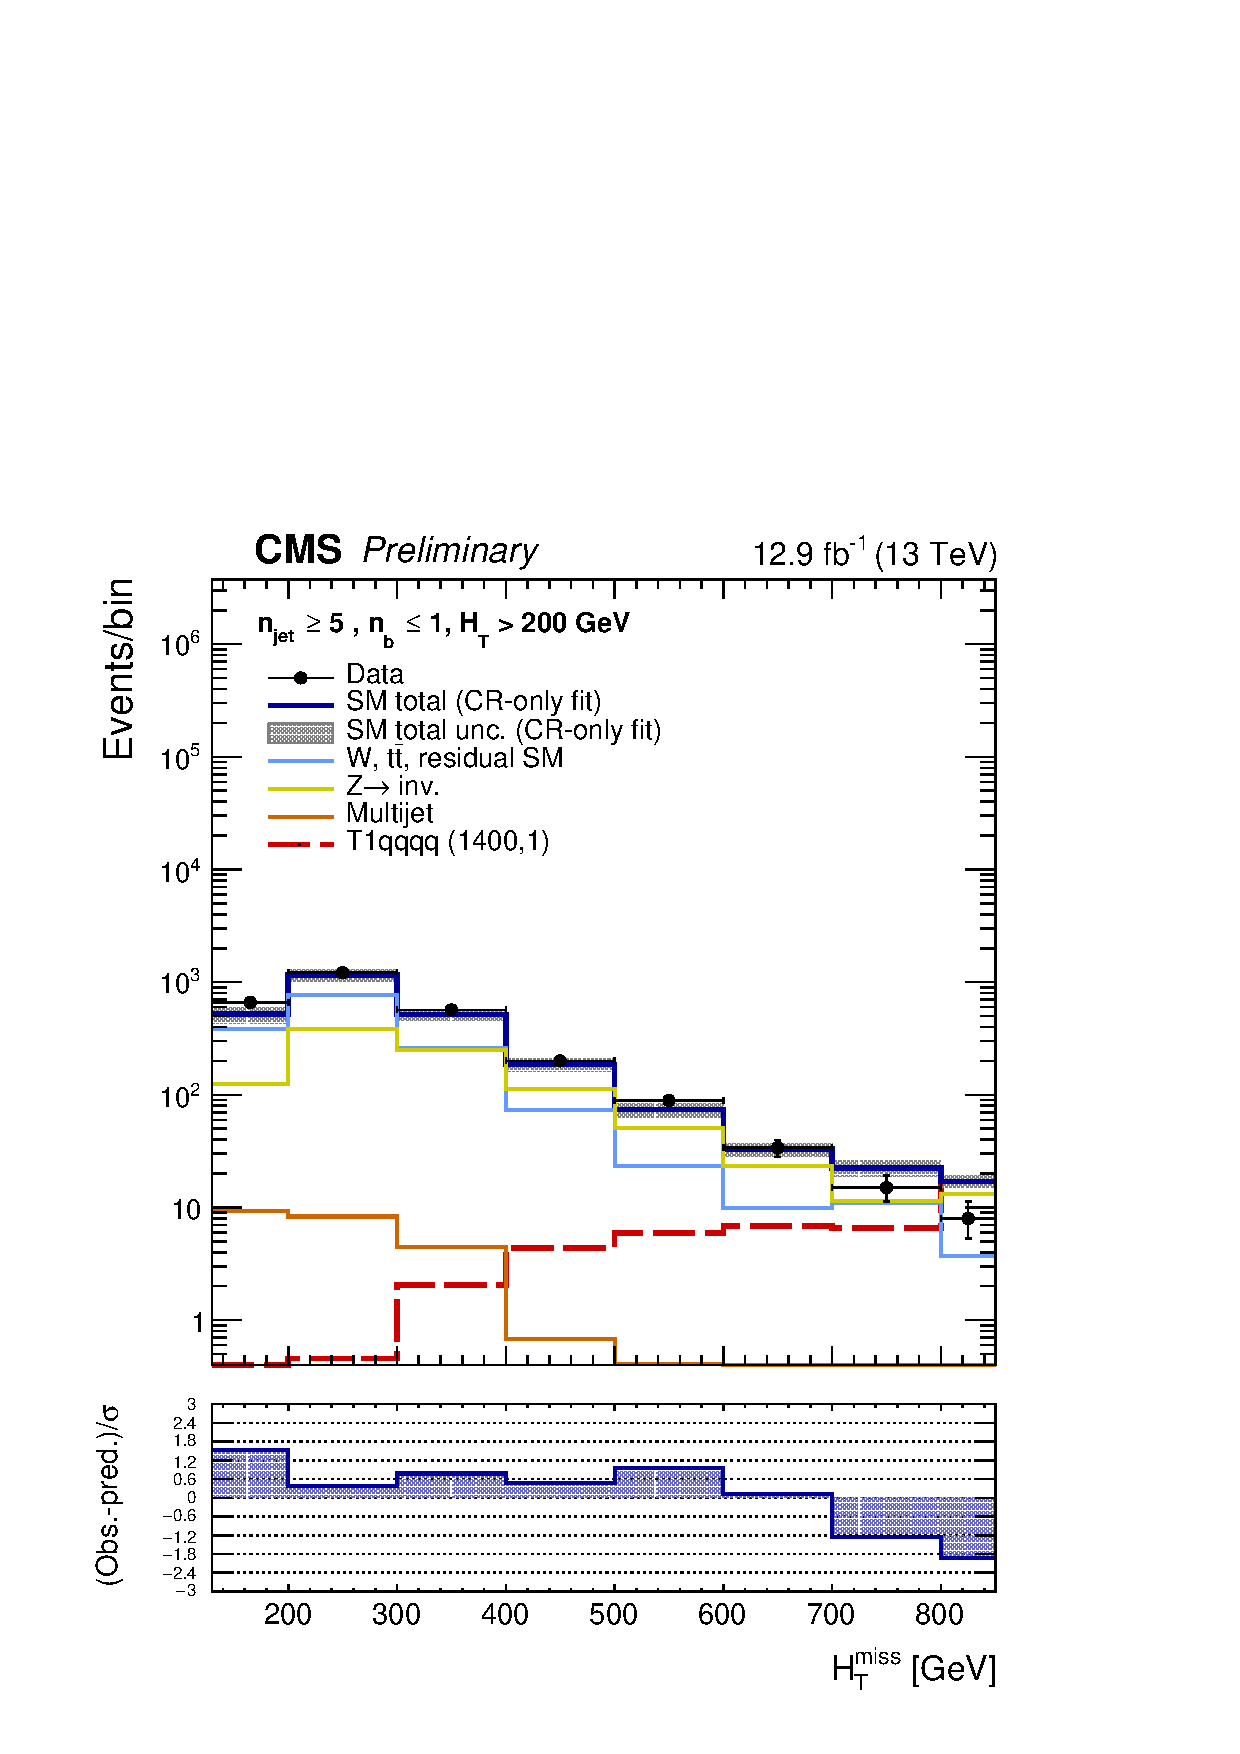
\includegraphics[width=0.4\textwidth]{figures/alphaT/agg_fitResults/mhtShape_le1b_ge5j_200_Inf_crfit_aux.pdf} } ~~
    \subfigure[High \nj, $\nb \geq 2$]{ 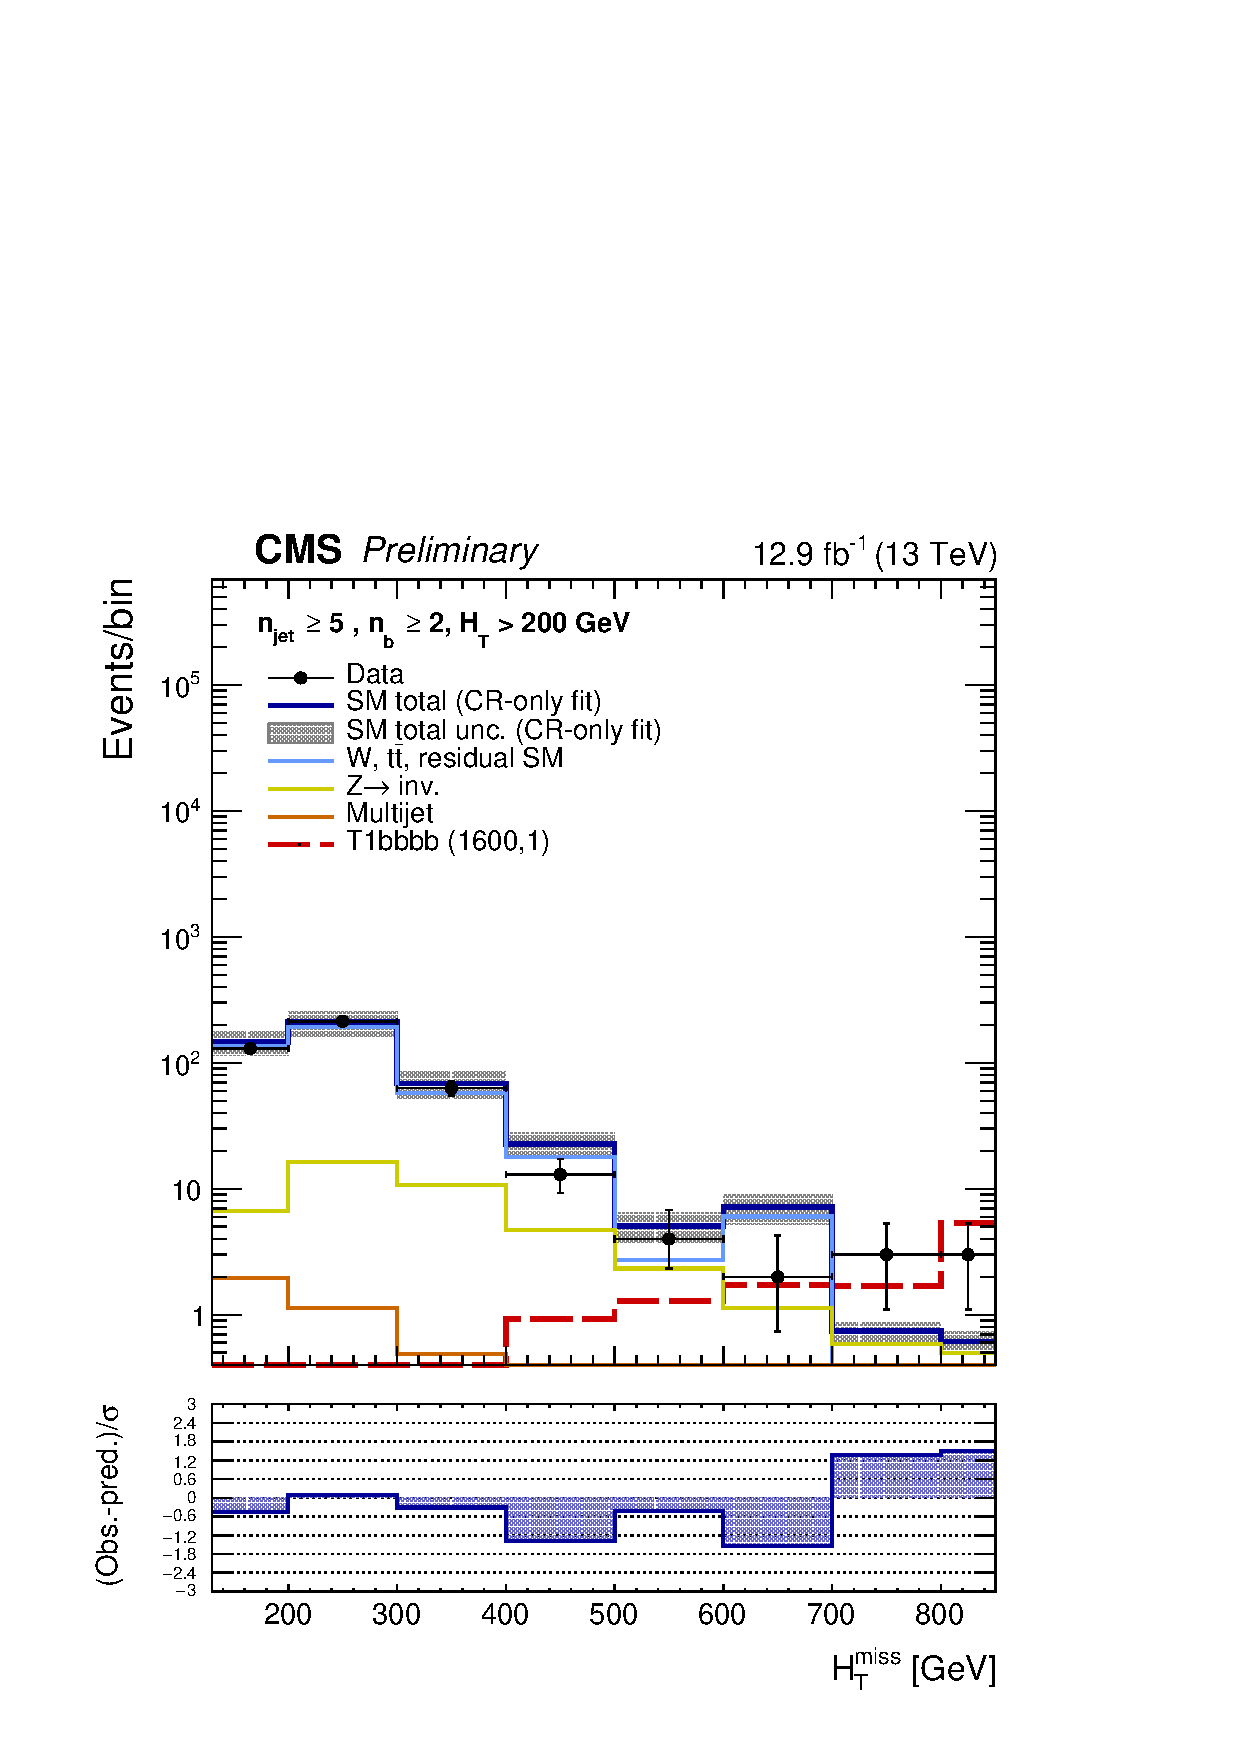
\includegraphics[width=0.4\textwidth]{figures/alphaT/agg_fitResults/mhtShape_ge2b_ge5j_200_Inf_crfit_aux.pdf} } \\
  \end{center}
\end{figure}


\clearpage
\begin{figure}[!tbhp]
    \caption{ Limit planes shown for both the full signal regions (left) and the aggregate regions (right).\label{fig:limit-planes}. 
    For the compressed models. }
  \begin{center}
    \subfigure[T2bb full signal region]{ 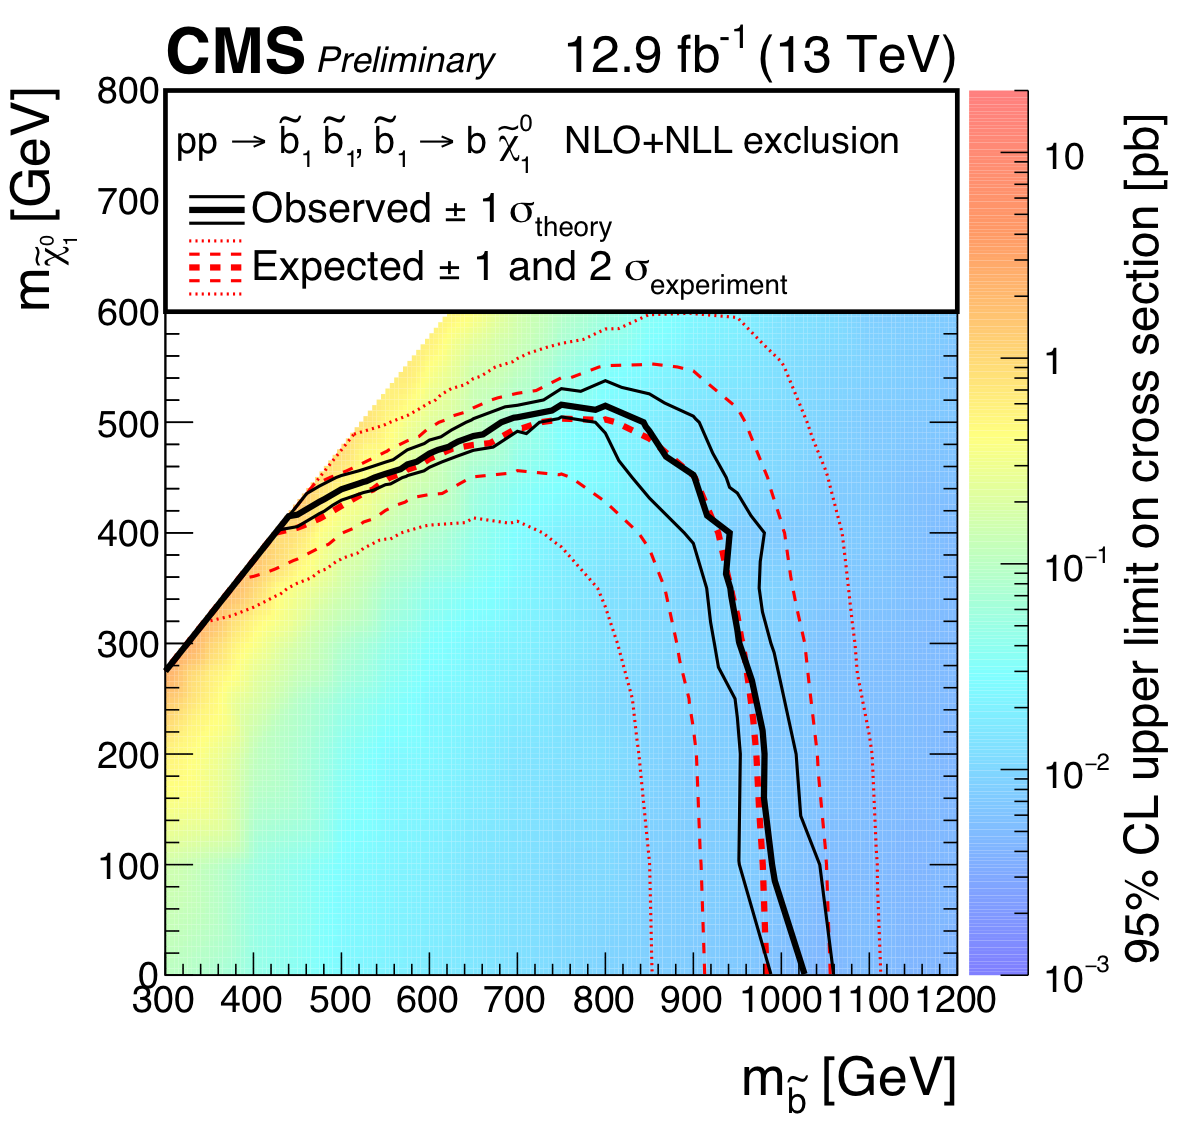
\includegraphics[width=0.45\textwidth]{figures//limitPlanesNominal/SUS16T2bbXSEC.png} } ~~
    \subfigure[T2bb aggregate regions]{ 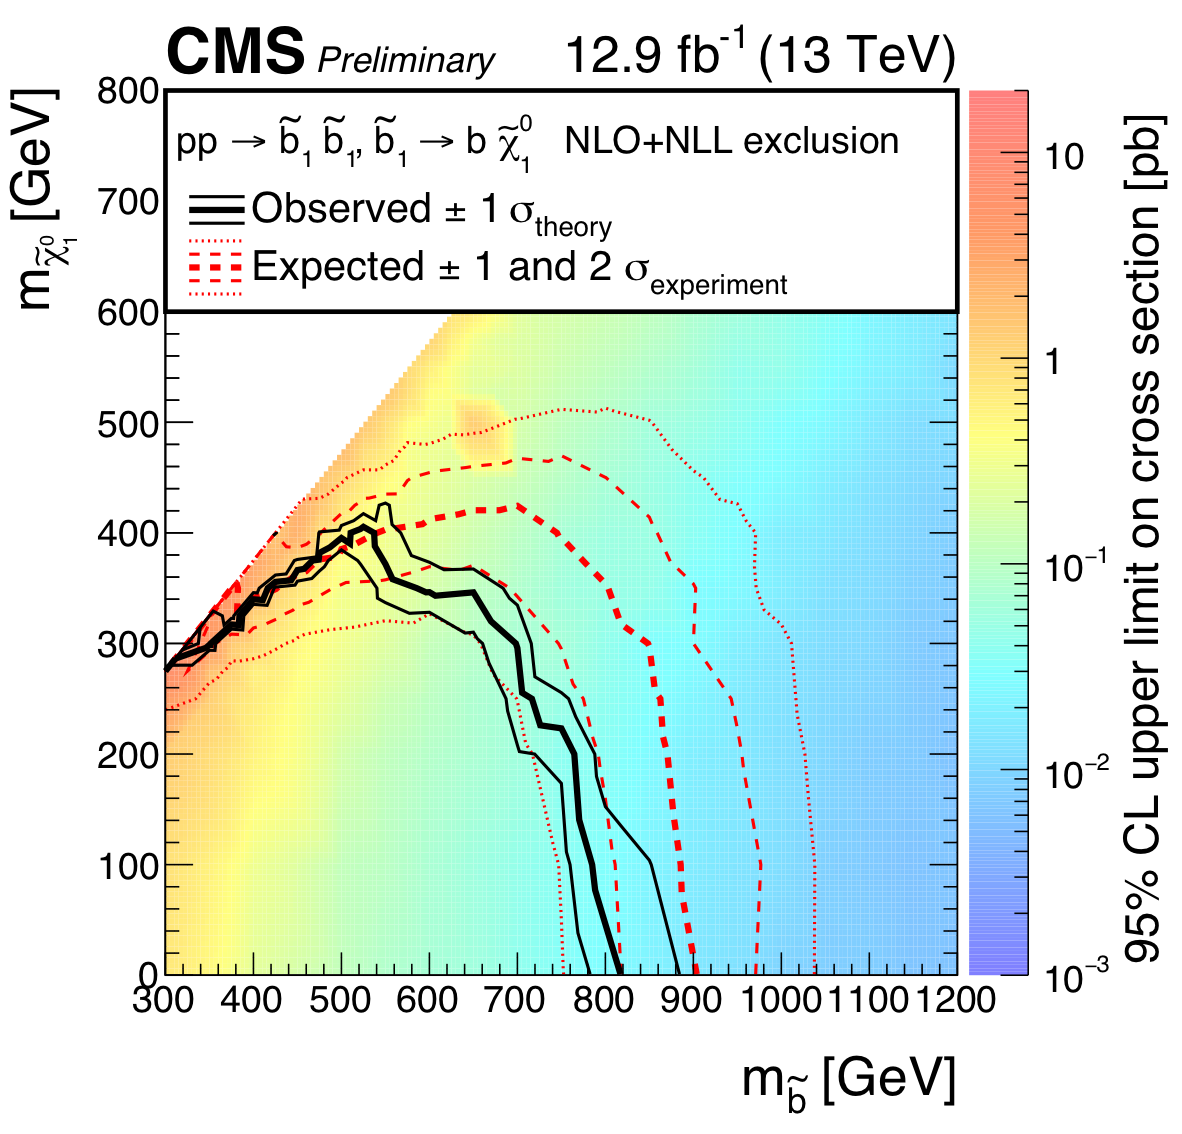
\includegraphics[width=0.45\textwidth]{figures//limitPlanesAgg/SUS16T2bbXSEC.png} } \\
    \subfigure[T2tt full signal region]   { 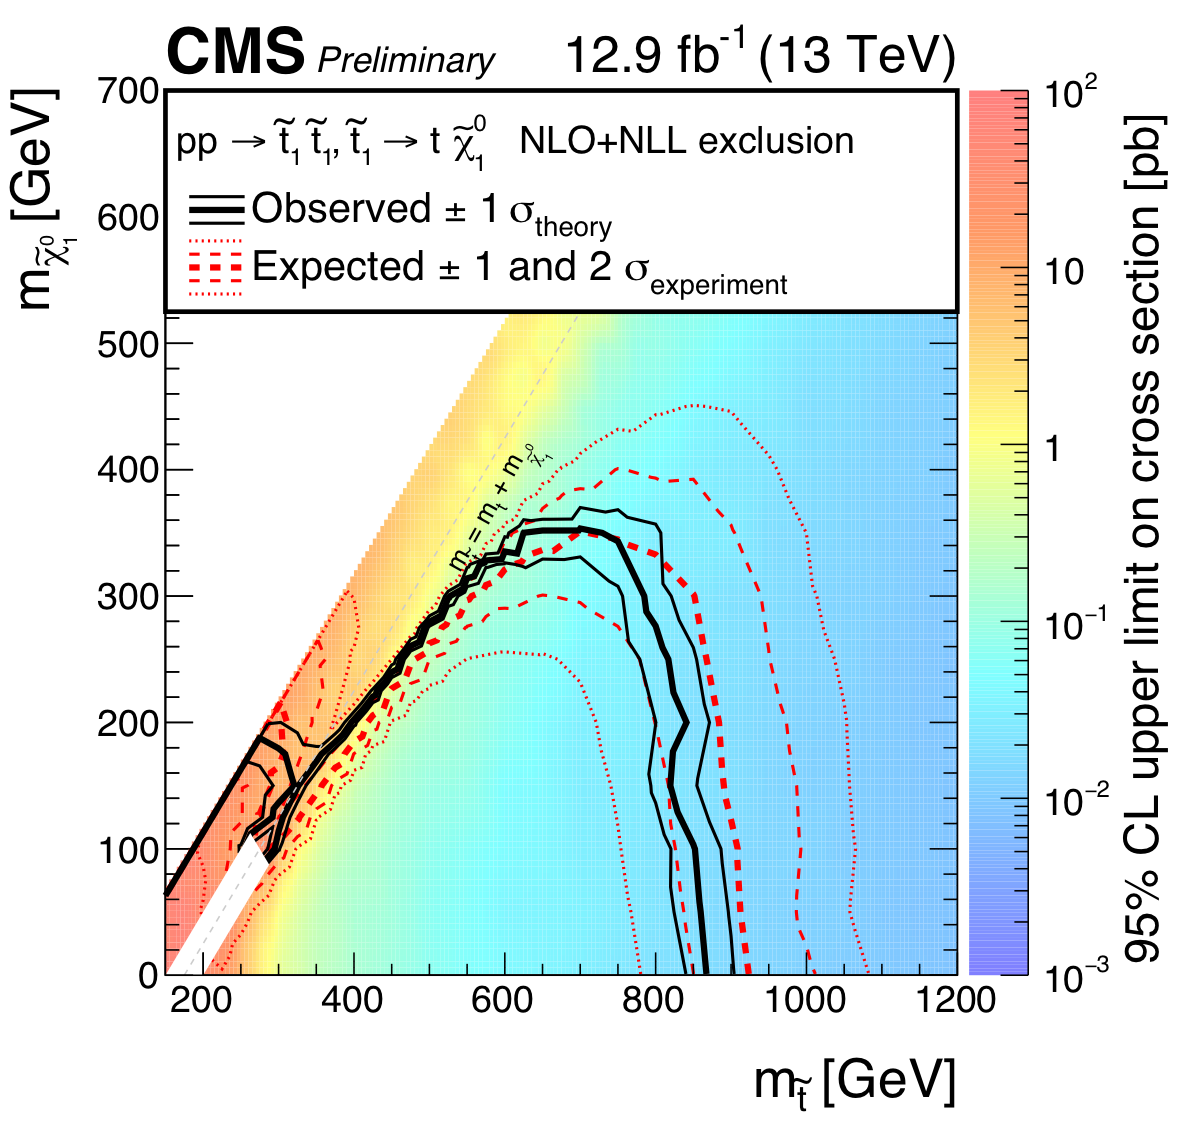
\includegraphics[width=0.45\textwidth]{figures//limitPlanesNominal/SUS16T2ttXSEC.png} } ~~
    \subfigure[T2tt aggregate regions]{ 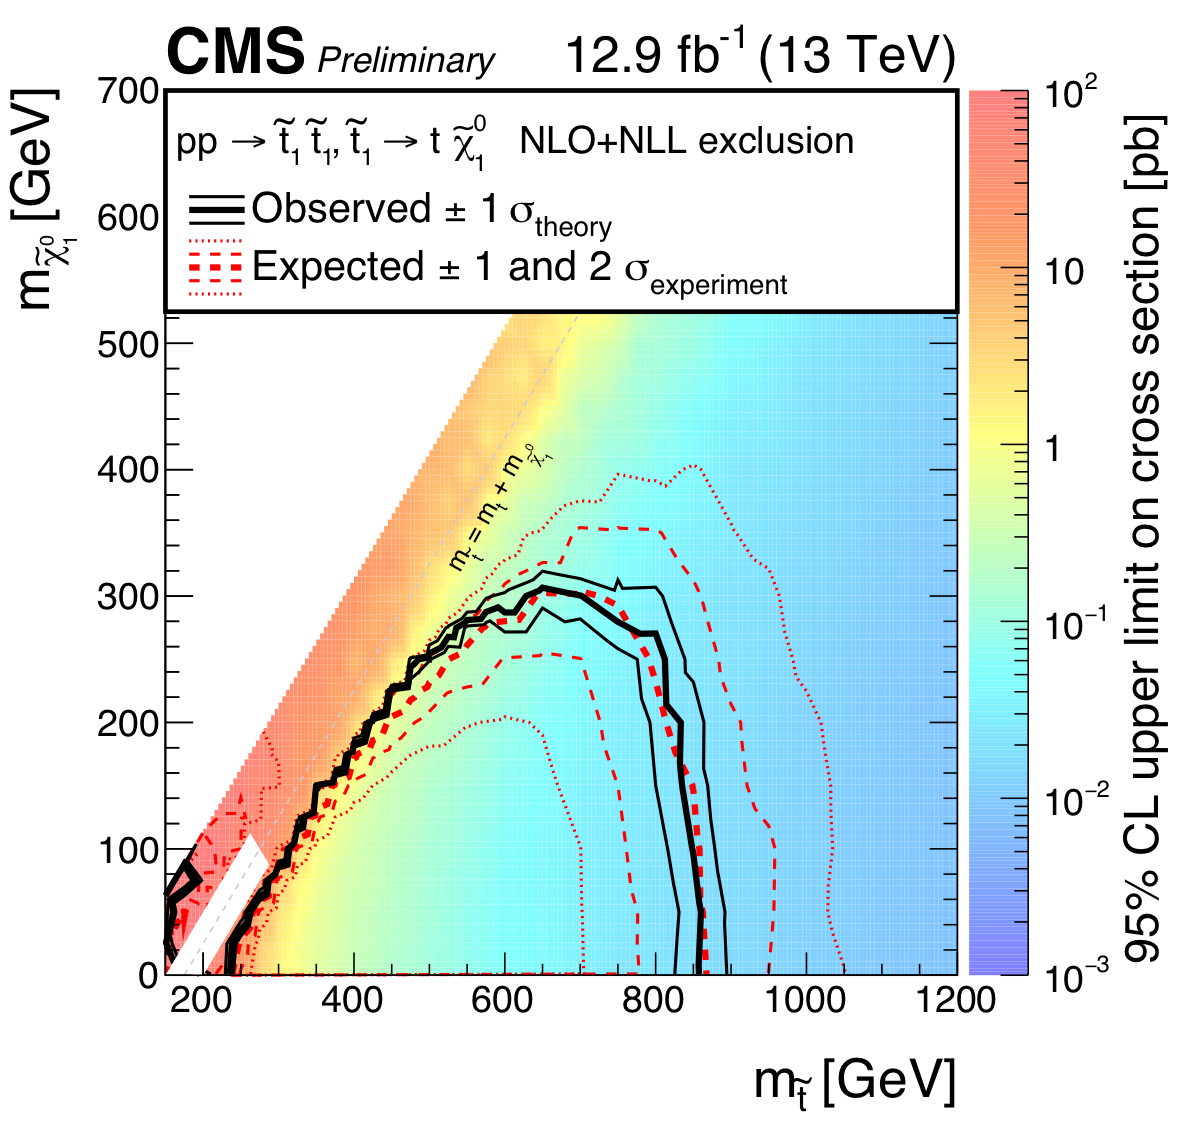
\includegraphics[width=0.45\textwidth]{figures//limitPlanesAgg/SUS16T2ttXSEC.png} } \\
    \subfigure[T1bbbb full signal region]   { 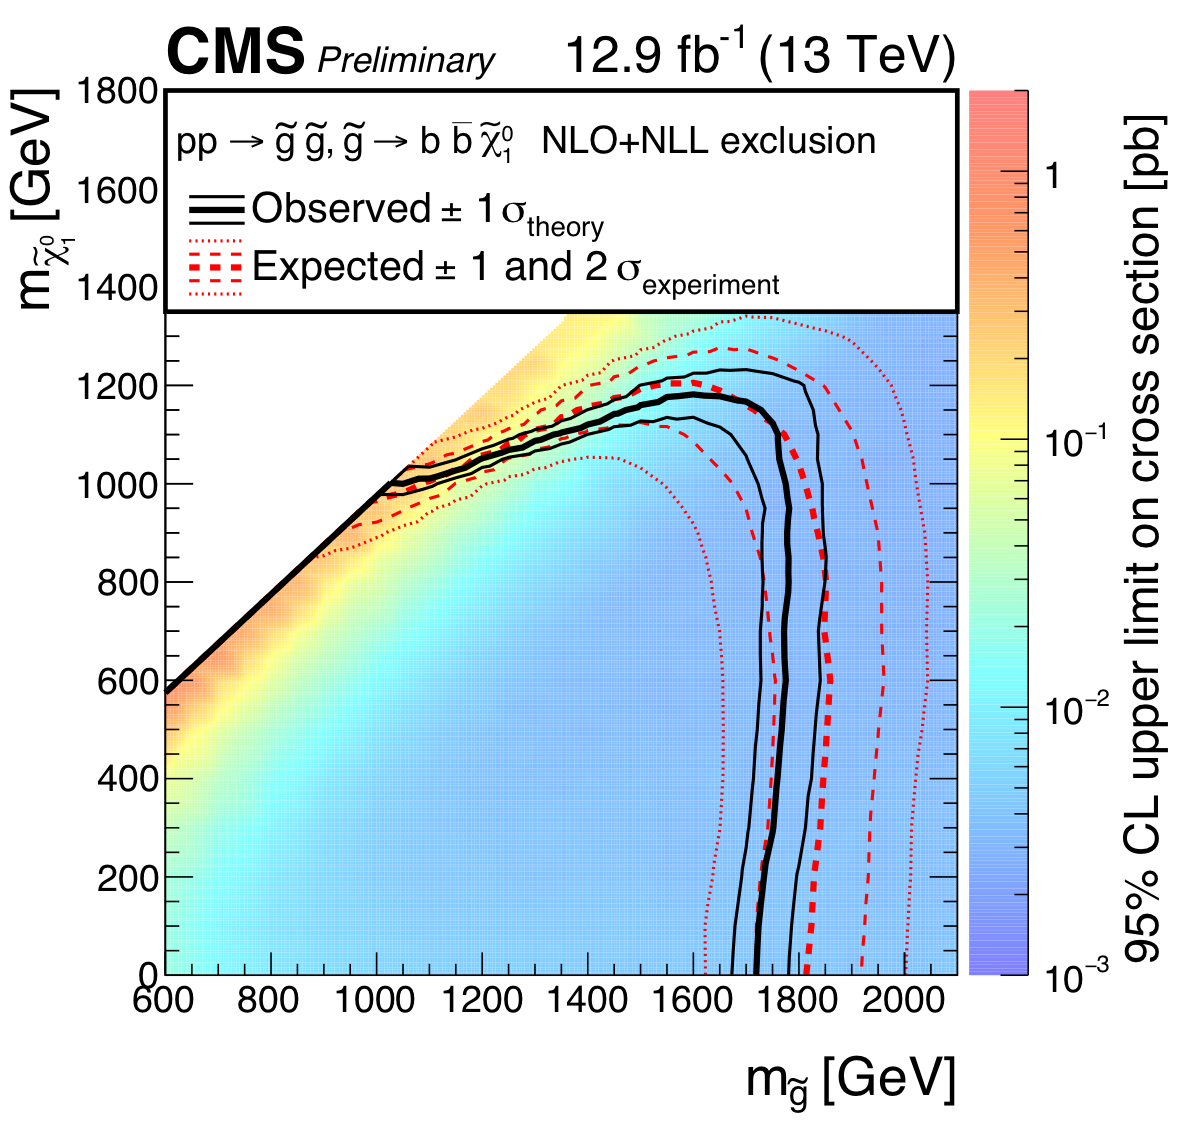
\includegraphics[width=0.45\textwidth]{figures//limitPlanesNominal/SUS16T1bbbbXSEC.png} } ~~
    \subfigure[T1bbbb aggregate regions]{ 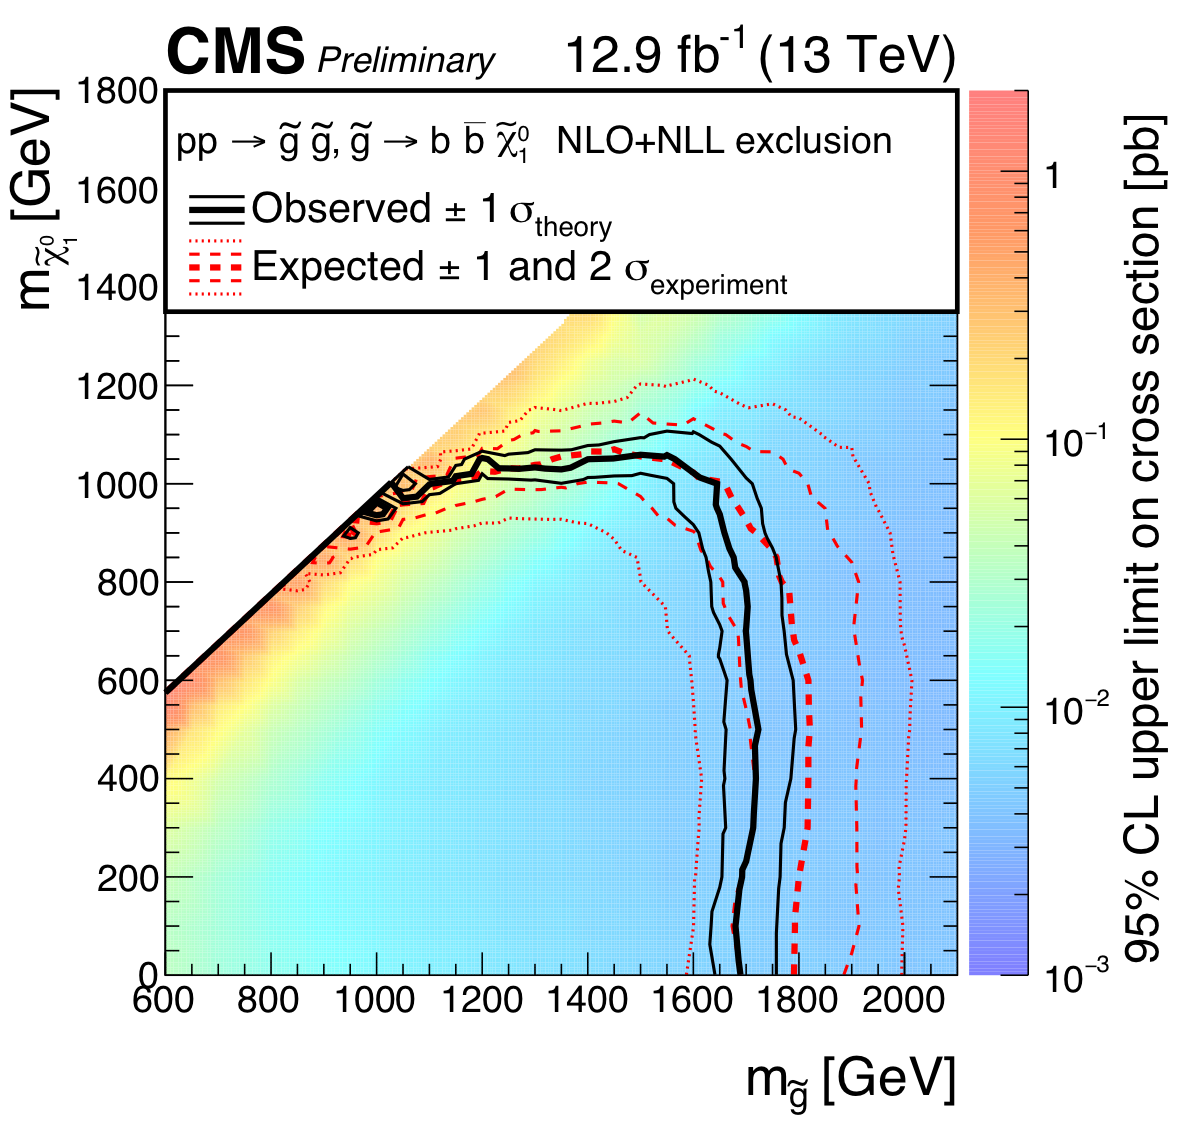
\includegraphics[width=0.45\textwidth]{figures//limitPlanesAgg/SUS16T1bbbbXSEC.png} } \\
  \end{center}
\end{figure}

\subsubsection{Validation of the simplified likelihood}

The covariance and predictions of the aggregate regions for the \alphat analysis may then 
be used to validate the simplified likelihood. Figure~\ref{fig:likelihoodscan-alphaT} 
shows the value of $q(\mu)$ as a function of $\mu$ for 
a benchmark model which has substantial contribution in many different signal regions 
(T2tt, mStop = 800, mLSP = 1). The values when $q(\mu)$ is defined using the likelihood of Equation~\ref{eq:full-likelihood} 
are shown and compared with the same definition but assuming no correlations between the 
background yields by setting $V_{ij}=0$ for $i\neq j$. The results using the full likelihood (with aggregate regions and no signal systematics) 
used by the \alphat analysis are also shown. The simplified likelihood shows good agreement with the full likelihood 
while it is clear that ignoring the correlations results in a bias of the estimate of $\hat{\mu}$. 

\begin{figure}[hbt]
  \begin{center} 
   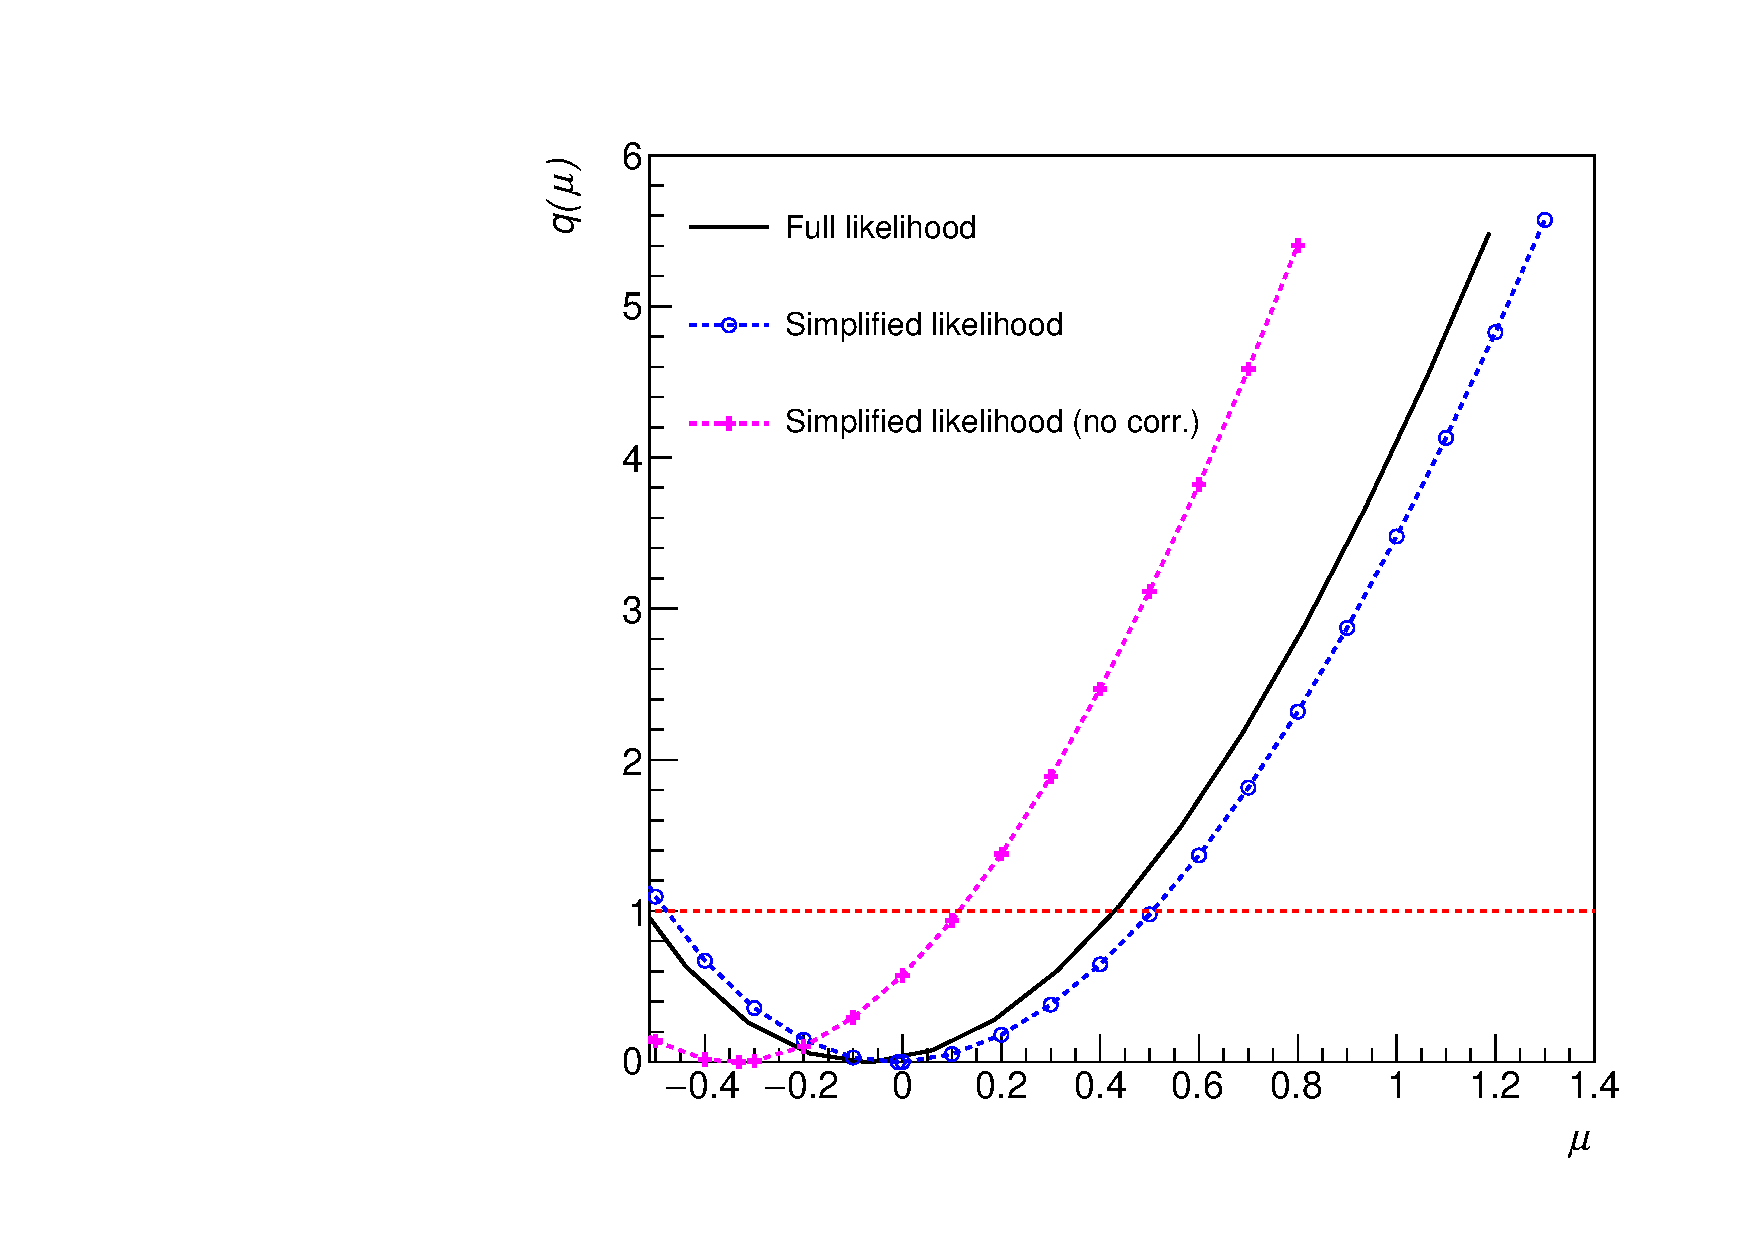
\includegraphics[width=1.5\cmsFigWidth]{figures/alphaT/rAT.pdf}
   \caption{The value of $q(\mu)$ for the \alphaT analysis defined using the simplified likelihood using the full covariance matrix (open blue points), assuming no correlations between the 
   background yields (open magenta crosses) and defined using the full likelihood (solid black line).}
   \label{fig:likelihoodscanAT} 
  \end{center}
\end{figure}

In Figure~\ref{fig:limitPlanes} the ratio between the limit with the simplified and the full likelihood is shown
for the simplified model T2bb. The contours of $\mu=1$ excluded at $95\%$ for the full likelihood, 
the simplified likelihood and the simplified likelihood where correlations are neglected are overlaid. When correlations
are considered the simplified and full likelihood provide comparable results, however, if 
these are neglected a significant bias is observed.

\begin{figure}[hbt]
  \begin{center} 
   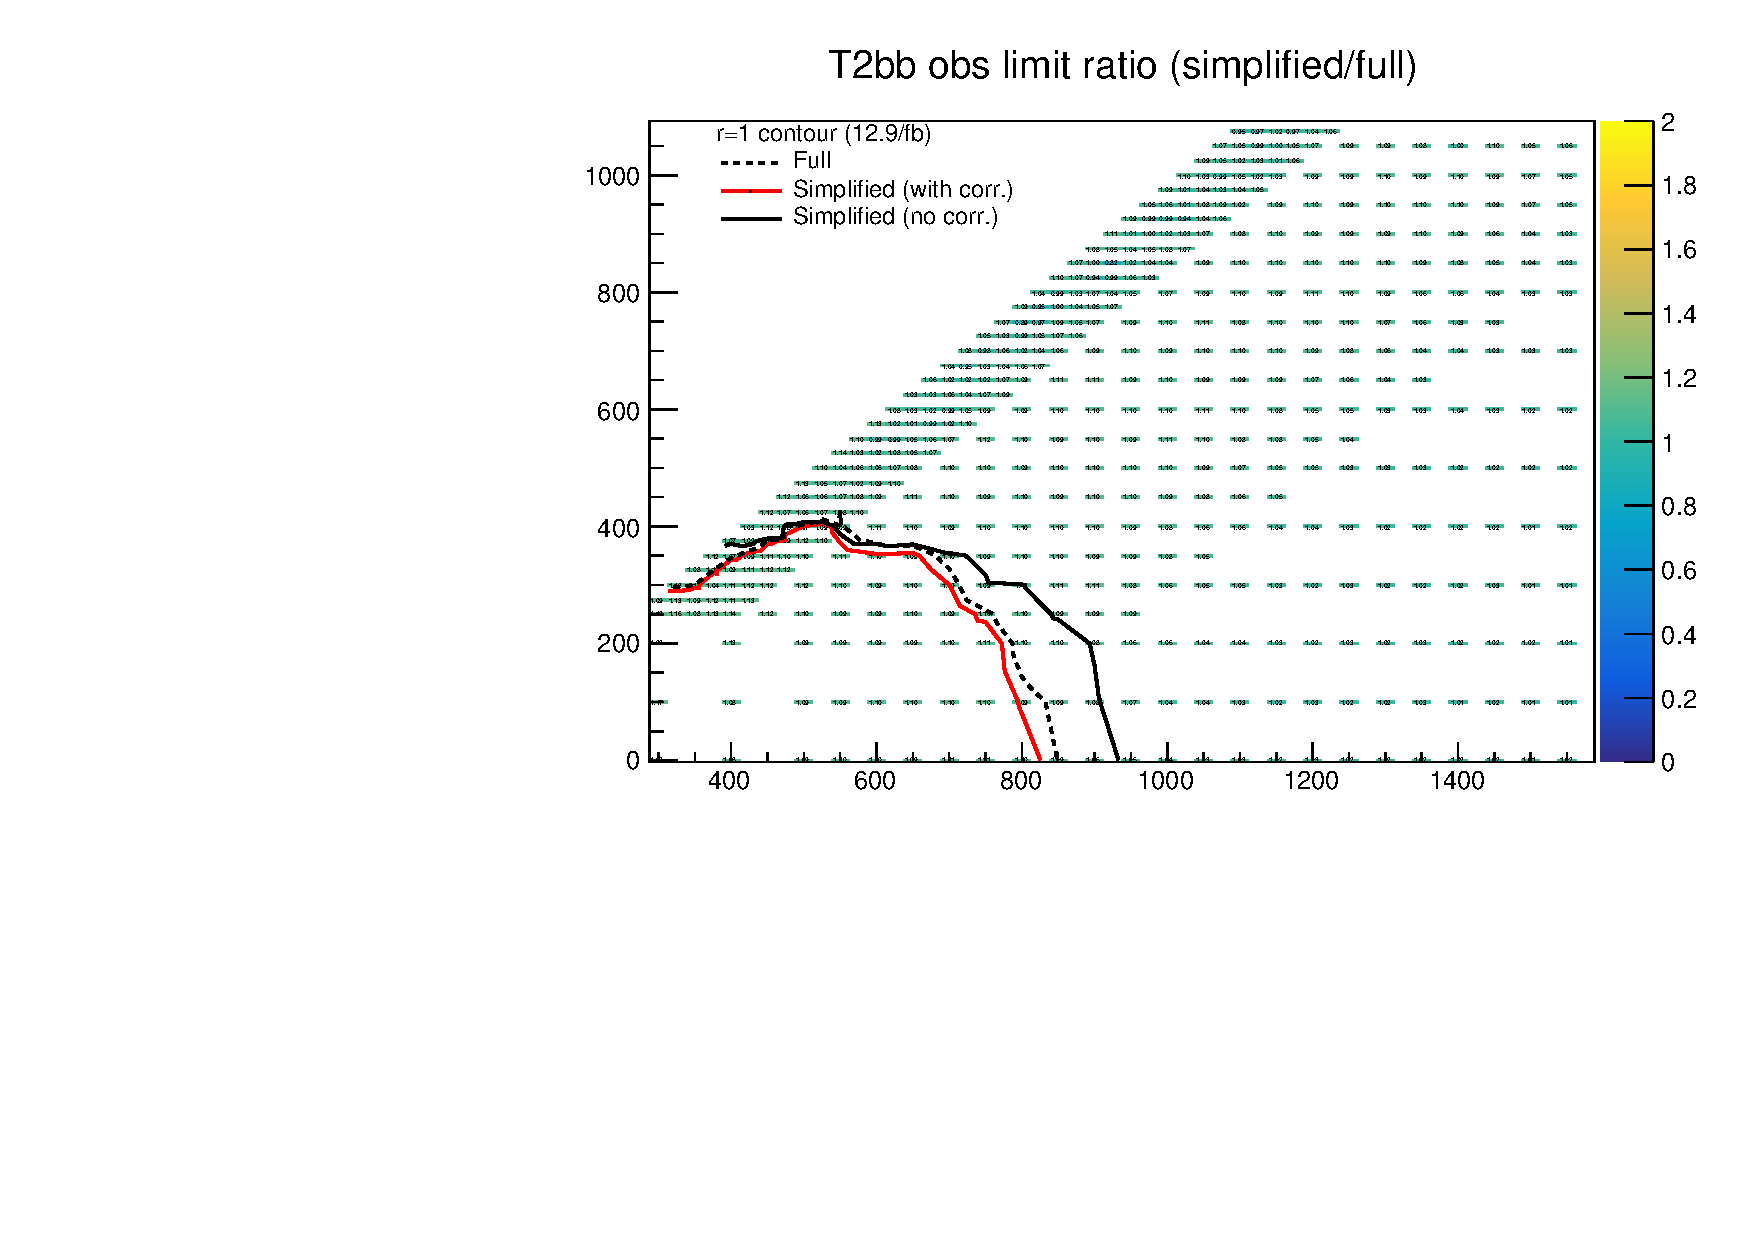
\includegraphics[width=1.5\cmsFigWidth]{figures/alphaT/full_T2bb_obs}
   \caption{Ratio of the $95\%$ upper limits for the simplified likelihood/full likelihood.
   The contour of $\mu=1$ for the simplified likelihood using the full covariance matrix (solid red line), 
   the simplified likelihood assuming no correlations between the background yields (solid black line) and the full
   likelihood (dotted black line) are overlaid.
   }
   \label{fig:limitPlanes} 
  \end{center}
\end{figure}
%%____________________________________________________________________________||






%%____________________________________________________________________________||



